%==============================================================
In the previous chapter, I explained the logical design of the MCS-4 chipset, comprising the \texttt{4004} (CPU), \texttt{4001} (ROM), \texttt{4002} (RAM), and \texttt{4003} (shift register). In this chapter, we construct a complete MCS-4 system by integrating these chips, and further reproduce the \texttt{141-PF} calculator developed by Busicom Corporation, implementing it on an FPGA. 

The user interfaces such as the calculator’s keyboard and printer, shown in Figure~\ref{fig:BUSICOM141PFKEYSW}, are realized using a modern microcontroller based on the RISC-V architecture, combined with a UART terminal or a Touch LCD panel. Our goal is to thoroughly appreciate the functionality and internal architecture of the historically significant \texttt{141-PF} calculator, which remains practically usable to this day and is exhibited in museums.

The RTL descriptions for the system are stored in the directory \texttt{RTL/}. The logic simulation stuffs can be found in the directory \texttt{SIM\_iverilog/} and \texttt{SIM\_questa/}. The FPGA implementation are stored in the directory \texttt{FPGA/}.

%----------------------------------
\begin{figure}[htbp]
  \includegraphics[width=1.0\textwidth]{./Figure/Busicom141PFKEYSW.png}
  \caption{Key Board and Switches on Calculator 141-PF}
  \label{fig:BUSICOM141PFKEYSW}
  \scriptsize{\textit{\url{https://www.flickriver.com/photos/gorekun/34947650073/}}}
\end{figure}
%----------------------------------

%==============================================================
\section{Overview of the designed MCS-4 System}
%--------------------------------------------------------------
This MCS-4 system is designed to emulate the configuration of the \texttt{141-PF} calculator, with the ultimate goal of implementation on an FPGA platform. The original \texttt{141-PF} calculator comprises five \texttt{4001} (ROM) chips—one of which is an optional chip for square root calculation routines—two \texttt{4002} (RAM) chips, three \texttt{4003} (shift register) chips, and a single \texttt{4004} (CPU) chip.

However, to accommodate pi calculation, which is described in another chapter, the memory architecture of the designed MCS-4 system has been expanded to its maximum configuration. Specifically, the \texttt{4004} (CPU) is connected to sixteen \texttt{4001} (ROM) chips and thirty-two \texttt{4002} (RAM) chips, organized into eight banks of four chips each.

A block diagram of the designed MCS-4 system is shown in Figure~\ref{fig:MCS4SYSTEMBLOCKDAGRAM}, and a specification summary is presented in Table~\ref{tb:MCS4SYSTEMSPEC}.

%----------------------------------
\begin{figure}[htbp]
  \centering
  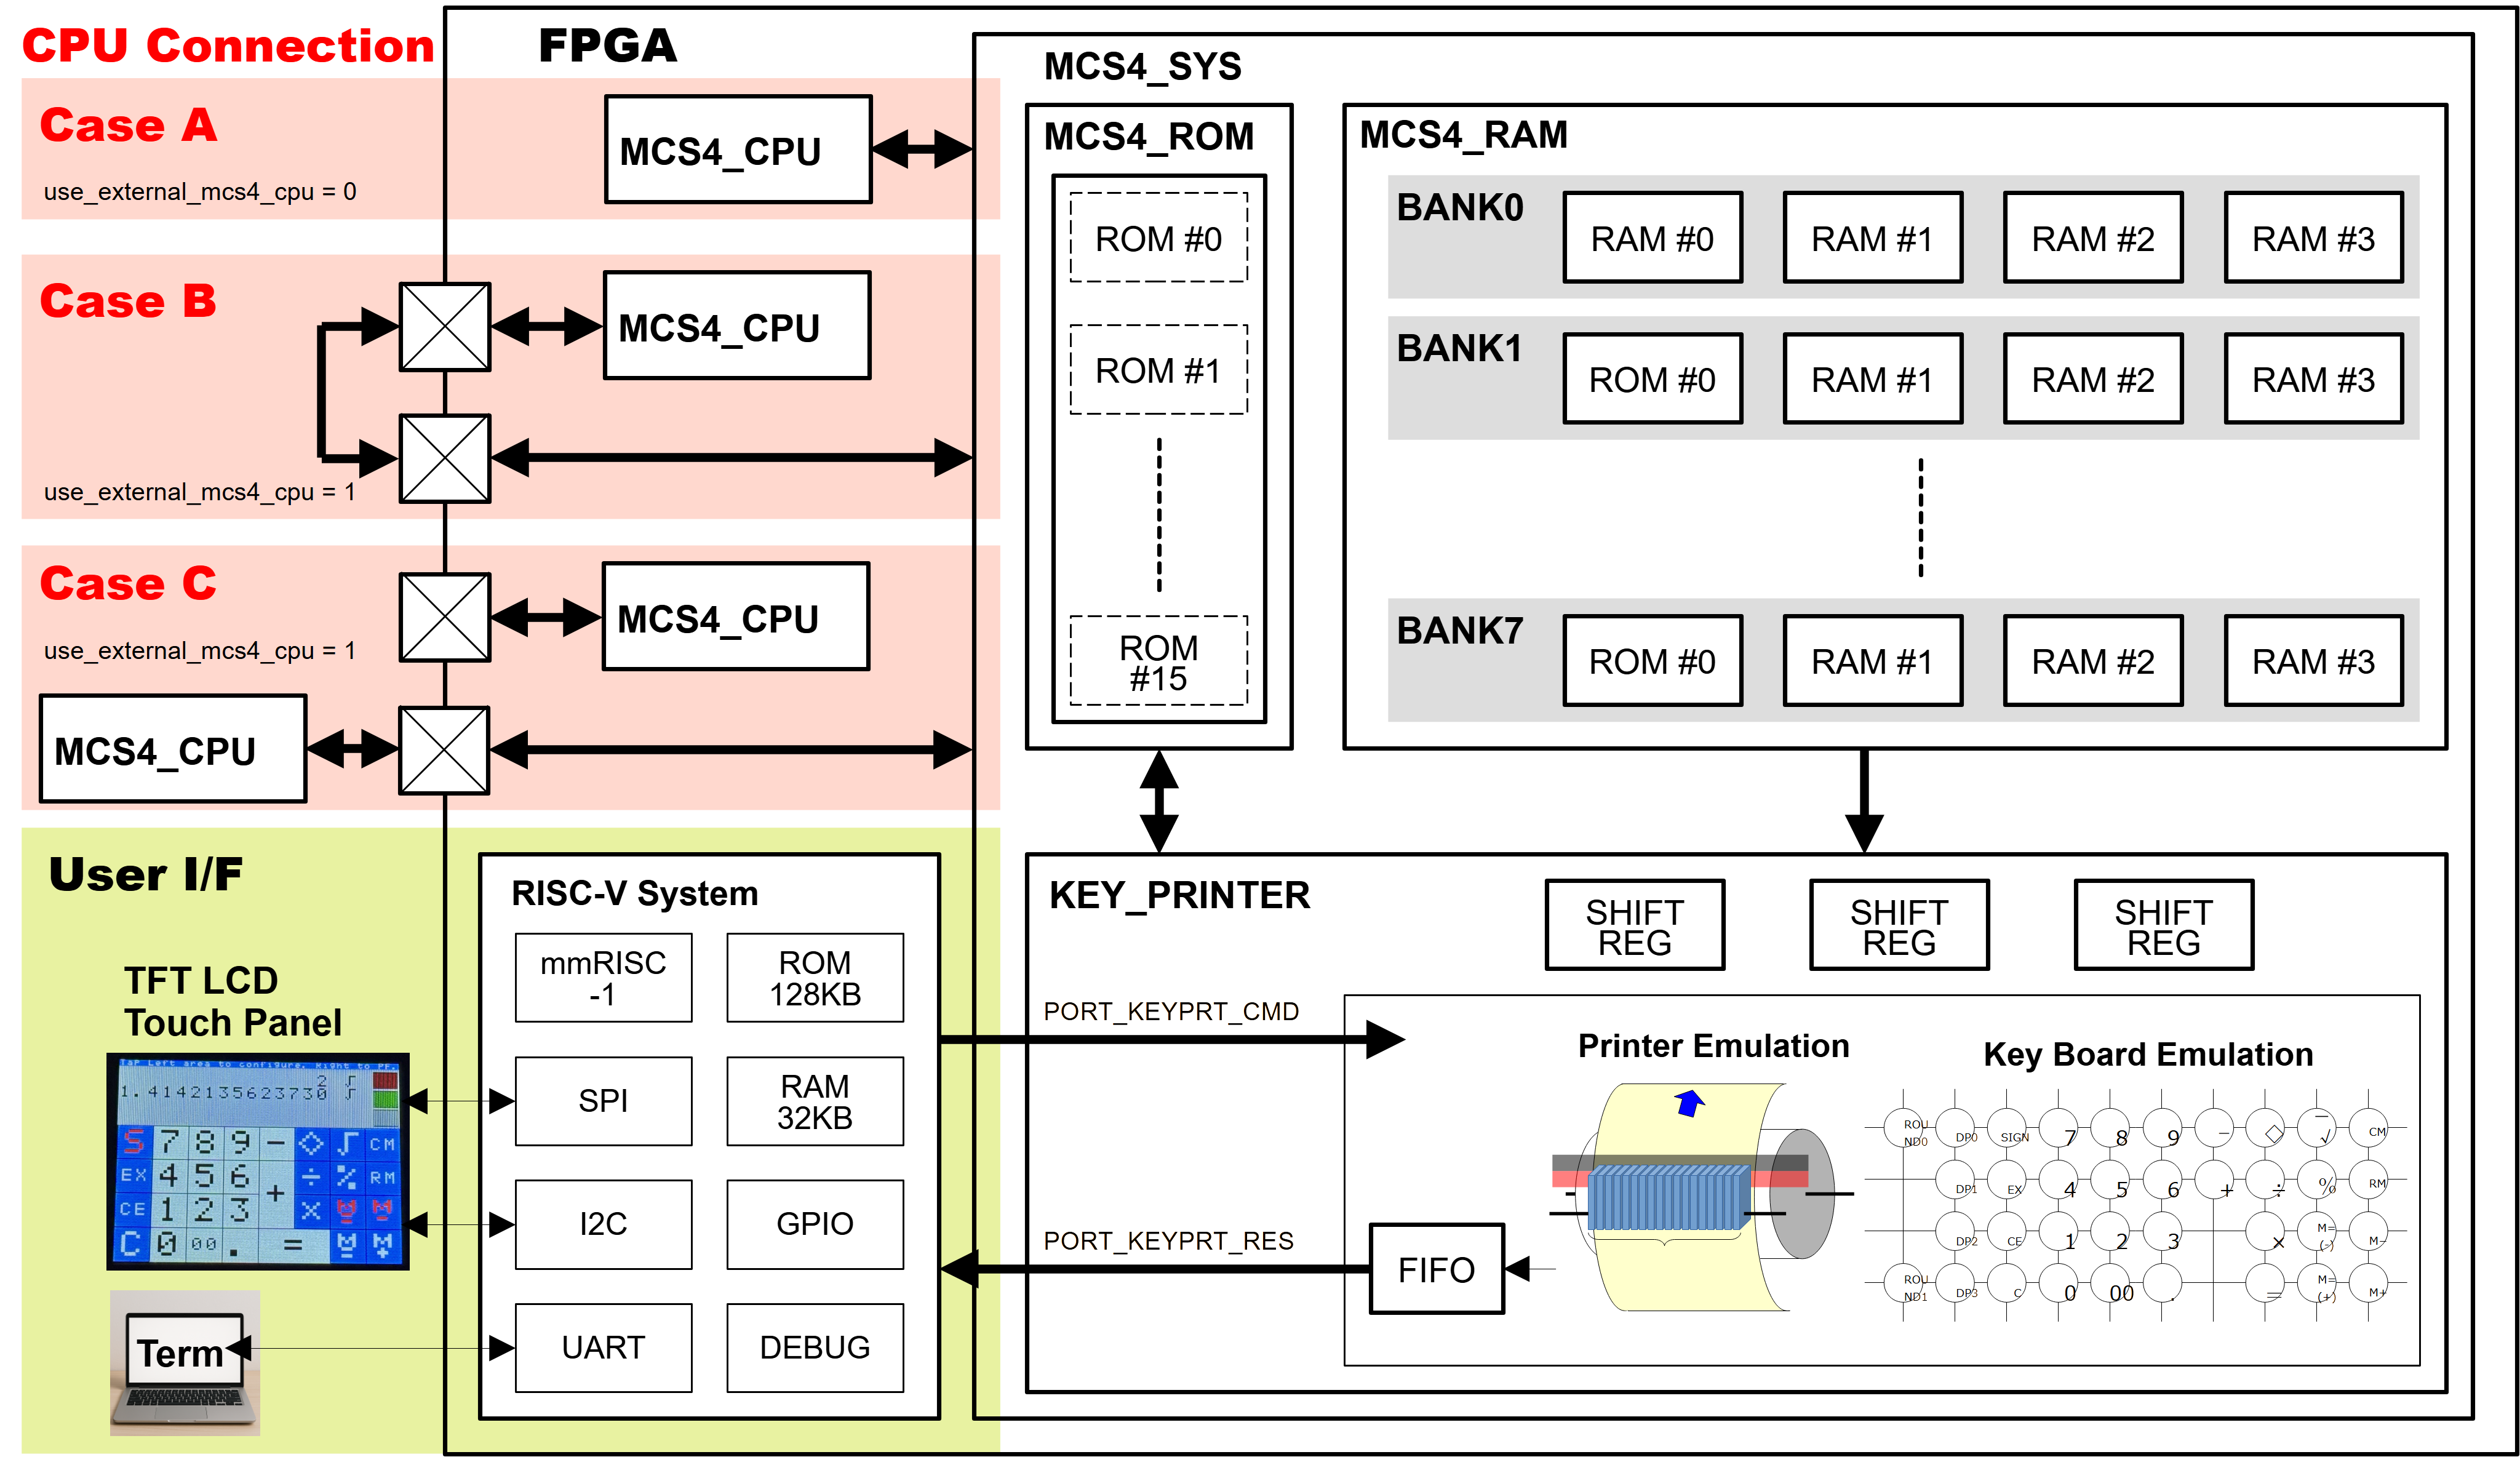
\includegraphics[width=1.0\textwidth]{./Figure/MCS4SystemBlockDiagram.png}
  \caption{Block Diagram of MCS-4 System}
  \label{fig:MCS4SYSTEMBLOCKDAGRAM}
\end{figure}
%----------------------------------
%----------------------------------
\begin{table}[htbp]
    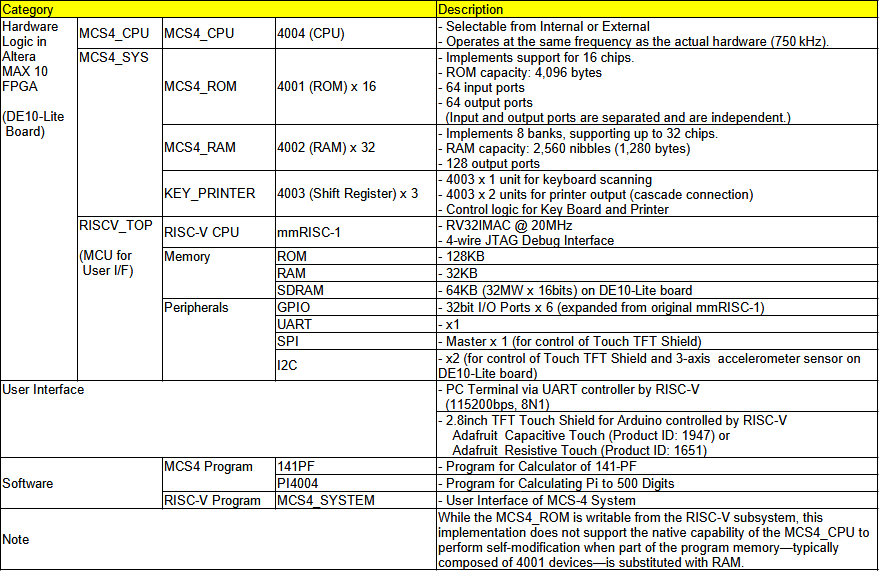
\includegraphics[width=1.00\columnwidth]{./Table/MCS4SystemSpec.png}
    \caption{MCS-4 System Specification}
    \label{tb:MCS4SYSTEMSPEC}
\end{table}
%----------------------------------

Peripheral circuitry of the MCS-4 system aligns with the hardware configuration of the \texttt{141-PF} calculator, utilizing three \texttt{4003} (shift register) chips. The behavior of the calculator's keyboard and printer interfaces is emulated using a modern RISC-V microcontroller system. The RISC-V subsystem adopts the existing \texttt{mmRISC-1} architecture, with peripheral functions retained and only the GPIO set extended\cite{mmRISC-1}.

Communication between the RISC-V subsystem and the MCS-4 system is handled via GPIO signals: command signals are transmitted through \texttt{PORT\_KEYPRT\_CMD[31:0]}, and responses are received through \texttt{PORT\_KEYPRT\_RES[31:0]}. The control logic for these command/response operations is implemented in the \texttt{KEY\_PRINTER} module, which also integrates three \texttt{4003} (shift register) chips.

User interaction via the RISC-V subsystem is primarily achieved through UART terminal operations. Optionally, a graphical interface is also available via a color LCD panel with touch functionality.

The \texttt{4004} (CPU) connects internally to the MCS-4 memory system (ROM and RAM) within the FPGA. Additionally, to accommodate the use of standalone \texttt{4004} chips, external connectivity is supported. Since the real \texttt{4004} chip is fabricated in a 10µm PMOS process and is electrically incompatible with the FPGA (due to voltage and DC level mismatches), external level-shifting circuitry might be required.

Nevertheless, recent advances in open-source PDKs and EDA tools have enabled free LSI designs, and users can fabricate a custom \texttt{4004} chip via low-cost foundry shuttle services. These chips can be connected to the FPGA and used for practical experimentation.

To support these scenarios, the FPGA design accommodates the following three configurations for CPU connection, selectable via onboard switches:

\begin{itemize}
  \item \textbf{Case A}: \texttt{4004} (CPU) connected internally to the FPGA's MCS-4 system (ROM and RAM)
  \item \textbf{Case B}: \texttt{4004} logic implemented in the FPGA, interfaced to the internal MCS-4 system via external pins
  \item \textbf{Case C}: Standalone \texttt{4004} chip connected via external pins to the FPGA's internal MCS-4 system (ROM and RAM)
\end{itemize}

Among these, Case~B and Case~C share an identical logical structure, differing only in their external connections. Case~B is provided as a debugging option for experimental use of Case~C.

%==============================================================
\section{FPGA Board and Optional Components Used}
%--------------------------------------------------------------
The MCS-4 system designed in this project is implemented on the DE10-Lite FPGA board from Teasic, as shown in Figure~\ref{fig:DE10LITE}. The DE10-Lite is a compact board equipped with an Altera MAX 10 FPGA. The user interface for the calculator application within this system is controlled by firmware running on a RISC-V subsystem embedded in the FPGA. This interface communicates with a terminal application on the PC via UART.\\

%----------------------------------
\begin{figure}[htbp]
  \centering
  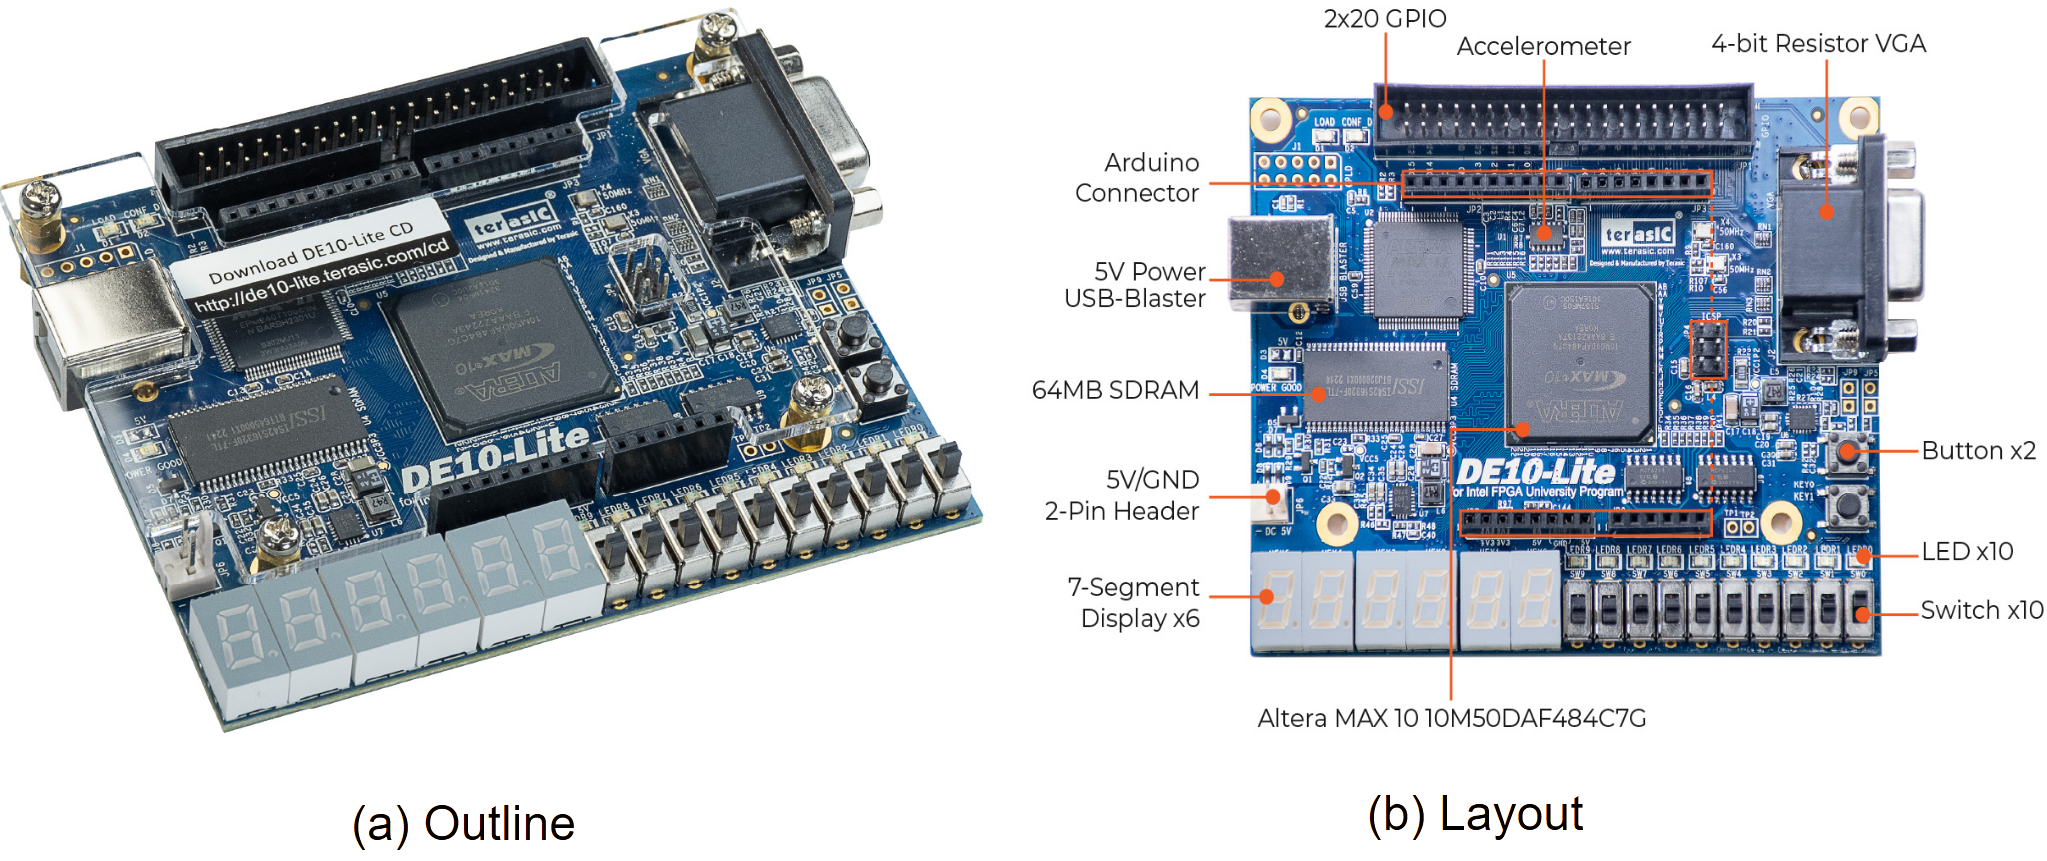
\includegraphics[width=1.0\textwidth]{./Figure/DE10LITE.png}
  \caption{Terasic DE10-Lite Board}
  \scriptsize{\textit{\url{https://www.terasic.com.tw/cgi-bin/page/archive.pl?Language=English&No=1021}}}
  \label{fig:DE10LITE}
\end{figure}
%----------------------------------

For users who prefer to operate the calculator via a graphical user interface (GUI), the system can be expanded by mounting an Arduino-compatible LCD panel with a capacitive touch screen onto the DE10-Lite board. The touch-enabled LCD panel used is the Adafruit 2.8" TFT Touch Shield for Arduino with Capacitive Touch (Product ID: 1947), as shown in Figure~\ref{fig:LCDPANELCAPACITIVE}.

The author also possesses a resistive touch panel variant of the LCD, shown in Figure~\ref{fig:LCDPANELCAPACITIVE}. This panel, the Adafruit 2.8" TFT Touch Shield for Arduino with Resistive Touch (Product ID: 1651), is also compatible with the system.

The firmware on the RISC-V subsystem automatically detects the presence of an LCD panel on the DE10-Lite board and the type of touch panel installed, switching the user interface from a UART-based terminal application to the touch-enabled LCD panel as appropriate.\\

However, the resistive touch panel version shown in Figure~\ref{fig:LCDPANELCAPACITIVE} has undergone a revision, and its integrated touch controller IC has been changed. Consequently, the latest model is not compatible with the firmware developed by the author.

%----------------------------------
\begin{figure}[htbp]
  \centering
  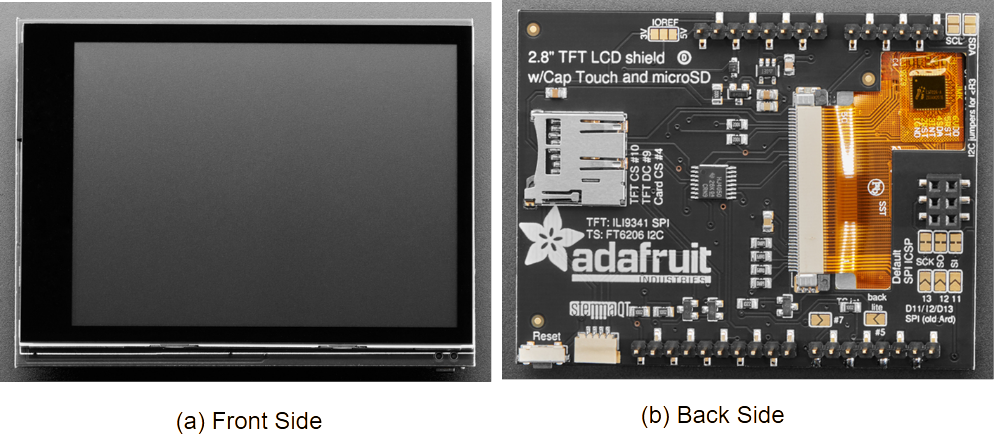
\includegraphics[width=0.75\textwidth]{./Figure/LCDPanelCapacitive.png}
  \caption{Adafruit 2.8" TFT Touch Shield for Arduino with Capacitive Touch (Product ID: 1947)}
  \textit{This is the recommended one. LCD Controller=ILI9341 (SPI I/F), Capacitive Touch Controller=FT6206 (I2C I/F).}\\
  \scriptsize{\textit{\url{https://www.adafruit.com/product/1947}}}
  \label{fig:LCDPANELCAPACITIVE}
\end{figure}
%----------------------------------
%----------------------------------
\begin{figure}[htbp]
  \centering
  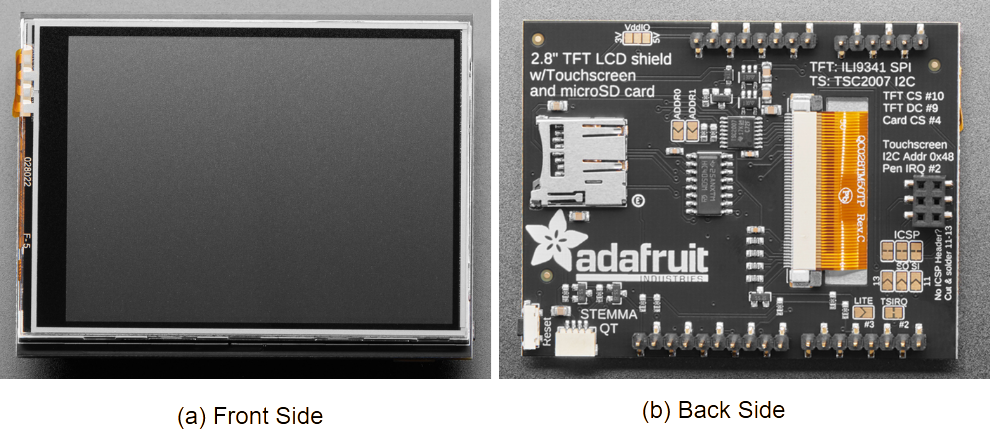
\includegraphics[width=0.75\textwidth]{./Figure/LCDPanelResistive.png}
  \caption{Adafruit 2.8" TFT Touch Shield for Arduino with Resistive Touch Screen (Product ID: 1651)}
  \textit{LCD Controller=ILI9341 (SPI I/F), Resistive Touch Controller=STMPE610 (SPI I/F).}\\
  \scriptsize{\textit{\url{https://www.adafruit.com/product/1651}}}
  \label{fig:LCDPANELRESISTIVE}
\end{figure}
%----------------------------------

%==============================================================
\section{Overview of the FPGA Top-Level Logic}
%--------------------------------------------------------------
The structure of the FPGA top-level logic is illustrated in Figure~\ref{fig:MCS4SYSTEMBLOCKDAGRAM}, and will be further explained in detail below. The top-level RTL description of the FPGA is located in \texttt{RTL/FPGA\_TOP/fpga\_top.v}, with the RTL description related to the MCS-4 system in \texttt{RTL/MCS4}, and the RISC-V subsystem in \texttt{RTL/RISCV}.
%--------------------------------------------------------------
\subsection{fpga\_top.v: FPGA Top-Level RTL Description}
Regarding the clock configuration, the 50\,MHz oscillator on the DE10-Lite board provides input to the FPGA, and the internal PLL generates a 20\,MHz clock for the RISC-V subsystem and a 750\,kHz clock for the MCS-4 system.

For the reset mechanism, a power-on reset generation circuit has been implemented within the FPGA. This consists of a counter that produces a reset signal with a fixed width. By setting synthesis constraints such that the counter is cleared to zero upon initial power-on, the reset behavior is reliably established. The final reset signal distributed inside the FPGA is synchronized by clock and constructed from an OR combination of the power-on reset signal, an external reset input from a switch, and the PLL lock signal.

%--------------------------------------------------------------
\subsection{Modules Related to MCS-4}
Within the top-level hierarchy of the FPGA, the \texttt{MCS4\_CPU} and \texttt{MCS4\_SYS} modules are instantiated. The \texttt{MCS4\_CPU} module represents the 4004 CPU, while the \texttt{MCS4\_SYS} module includes the \texttt{MCS4\_ROM}, \texttt{MCS4\_RAM}, and \texttt{KEY\_PRINTER} modules.

As described in the previous section, three configurations—Case A, Case B, and Case C—are available for connecting the \texttt{MCS4\_CPU}, and the selection logic is also implemented within the top-level hierarchy. Specifically, the external SW9 switch input is connected via \texttt{GPIO2[9]} and captured as the signal \texttt{use\_external\_mcs4\_cpu}. When this signal level is Low, Case A is selected; when High, either Case B or Case C is enabled. This switching mechanism is the reason why \texttt{MCS4\_CPU} and \texttt{MCS4\_SYS} modules are separated.

Table~\ref{tb:SIGNALSMCS4SYS} lists the input/output signals of the \texttt{MCS4\_SYS} module, while Table~\ref{tb:SIGNALSKEYPRINTER} summarizes the input/output signals of the \texttt{KEY\_PRINTER} module.

%----------------------------------
\begin{table}[htbp]
    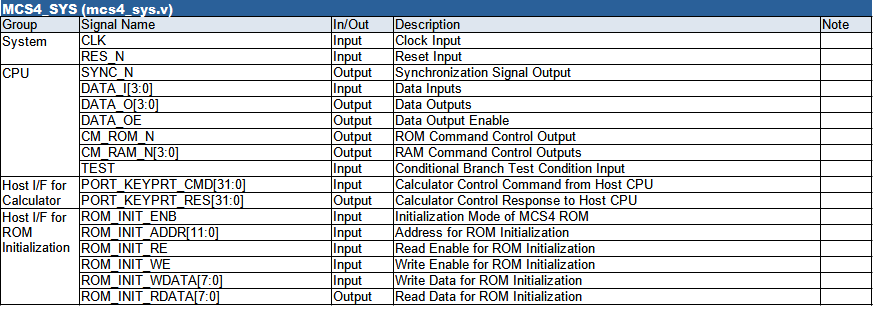
\includegraphics[width=1.00\columnwidth]{./Table/SignalsMCS4SYS.png}
    \caption{I/O Signals of \texttt{MCS4\_SYS}}
    \label{tb:SIGNALSMCS4SYS}
\end{table}
%----------------------------------
%----------------------------------
\begin{table}[htbp]
    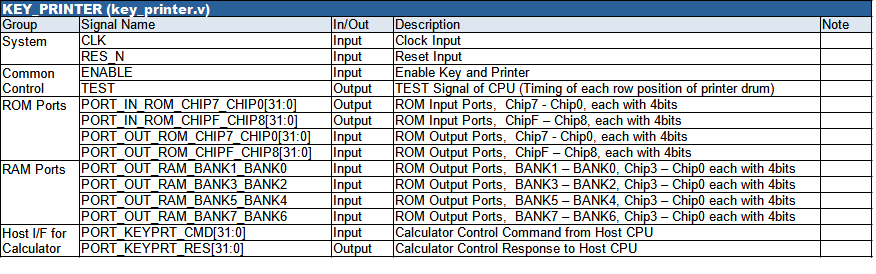
\includegraphics[width=1.00\columnwidth]{./Table/SignalsKEYPRINTER.png}
    \caption{I/O Signals of \texttt{KEY\_PRINTER}}
    \label{tb:SIGNALSKEYPRINTER}
\end{table}
%----------------------------------

%--------------------------------------------------------------
\subsection{RISC-V Subsystem}
The RISC-V subsystem utilizes the mmRISC-1\cite{mmRISC-1} design as-is, including its peripheral functions. However, the original configuration of three 32-bit GPIO ports has been expanded to six ports in this system.

%==============================================================
\section{Logic Description of MCS-4 Related Modules}
%--------------------------------------------------------------
The \texttt{MCS4\_CPU} module is a faithful implementation of the Intel 4004 CPU, which is described in detail in a separate chapter. The \texttt{MCS4\_SYS} module comprises the \texttt{MCS4\_ROM}, \texttt{MCS4\_RAM}, and \texttt{KEY\_PRINTER} modules, with each ROM and RAM module also explained in a separate section. This chapter focuses on the \texttt{KEY\_PRINTER} module.

%--------------------------------------------------------------
\subsection{KEY\_PRINTER Module}
The \texttt{KEY\_PRINTER} module integrates three 4003 shift registers, forming a circuit that emulates the keyboard, printer, and status indicator lamps of the calculator. It connects to the input/output ports of the \texttt{MCS4\_ROM} module and to the output ports of the \texttt{MCS4\_RAM} module, thereby simulating the behavior of the original 141-PF calculator.

This module also interfaces with a RISC-V subsystem responsible for user interaction. It exchanges command and response signals through \texttt{PORT\_KEYPRT\_CMD[31:0]} and \texttt{PORT\_KEYPRT\_RES[31:0]}, respectively. Operating at 750 kHz, the \texttt{KEY\_PRINTER} faithfully reproduces the speed and performance of the original 141-PF calculator hardware.

%--------------------------------------------------------------
\subsection{I/O Circuitry of Busicom 141-PF}
The \texttt{KEY\_PRINTER} module emulates the I/O circuits located outside the ROM (4001) and RAM (4002) ports of the 141-PF calculator. This emulation allows the original Busicom binary code, available online, to execute correctly. Figure~\ref{fig:IOBLOCK141PF} illustrates the external I/O circuitry assumed by the 141-PF program.

To expand the number of output ports, this circuit uses multiple 4003 shift registers. Table~\ref{tb:ROMRAMPORT} lists the connection targets for the ROM/RAM I/O ports, while Table~\ref{tb:USAGE4003} shows the configuration of 4003 shift registers within the calculator’s I/O circuitry.

%----------------------------------
\begin{figure}[htbp]
  \centering
  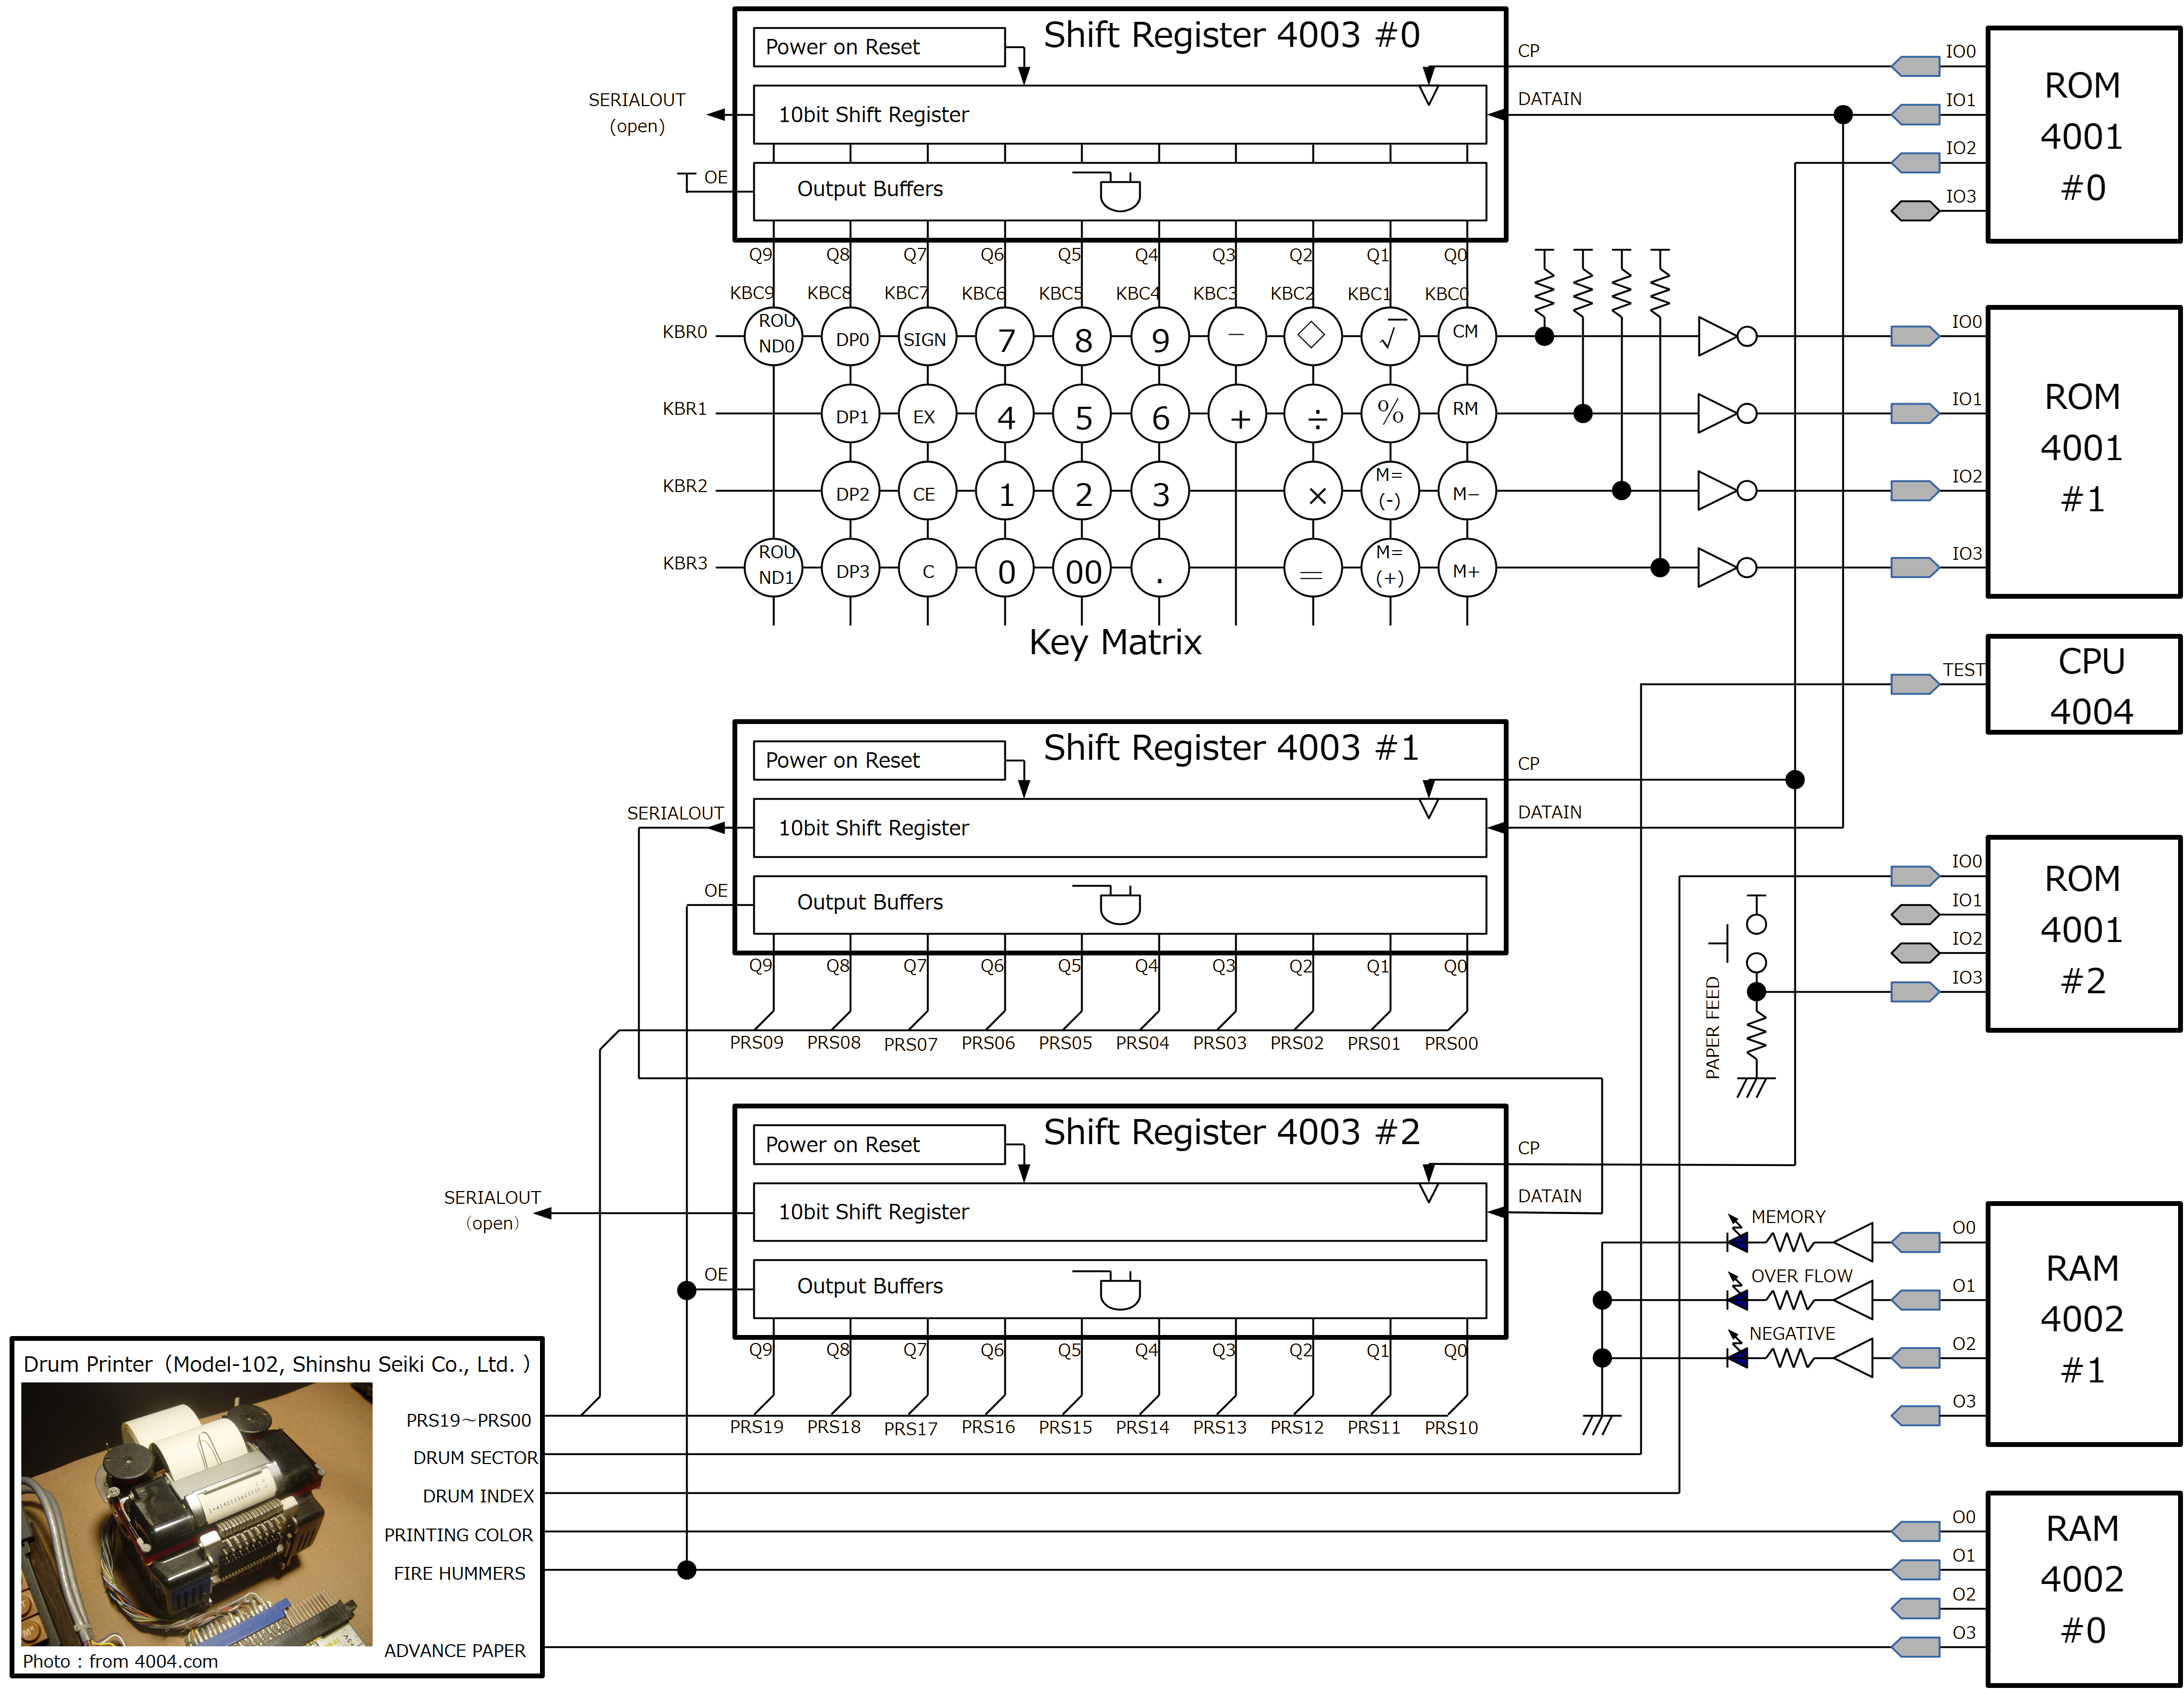
\includegraphics[width=1.0\textwidth]{./Figure/IOBlock141PF.png}
  \caption{I/O Circuit of the Busicom 141-PF Calculator via MCS-4 System}
  \label{fig:IOBLOCK141PF}
\end{figure}
%----------------------------------
%----------------------------------
\begin{table}[htbp]
    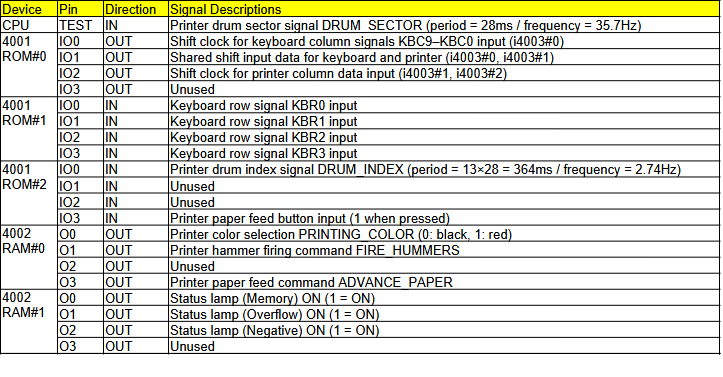
\includegraphics[width=1.00\columnwidth]{./Table/ROMRAMPort.png}
    \caption{Connections of ROM/RAM I/O Ports in the Calculator I/O Circuit}
    \label{tb:ROMRAMPORT}
\end{table}
%----------------------------------
%----------------------------------
\begin{table}[htbp]
    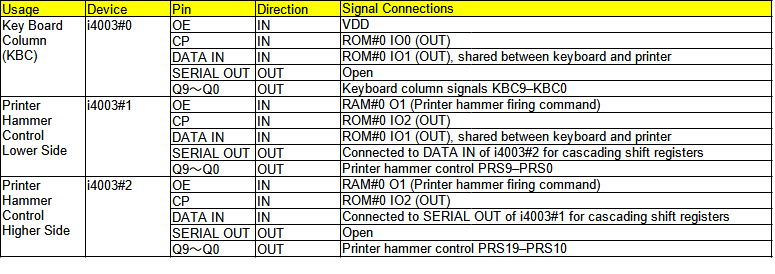
\includegraphics[width=1.00\columnwidth]{./Table/Usage4003.png}
    \caption{Connection Method of 4003 Registers Within the Calculator I/O Circuit}
    \label{tb:USAGE4003}
\end{table}
%----------------------------------

%--------------------------------------------------------------
\subsection{Keyboard Matrix of the Calculator}
The keyboard of the Busicom 141-PF calculator, along with the input switches (rounding mode selector and decimal digit selector), is read via a matrix circuit. When a key or switch is activated, its intersection connects a column signal (KBC0 to KBC9) with a row signal (KBR0 to KBR3).

As shown at the top of Figure~\ref{fig:IOBLOCK141PF}, the 4003 \#0 shift register generates the KBC0–KBC9 column signals. The clock and shift input data for 4003 \#0 are supplied from IO0 and IO1 of 4001 (ROM) \#0, respectively.

The four row signals KBR0–KBR3 are read via pull-up resistors and inverters through the input ports of 4001 (ROM) \#1. When no keys are pressed, all four signals read LOW by 4001 (ROM) \#1. The column signals KBC0–KBC9 are initially set to HIGH, and each is momentarily pulled LOW in sequence at high speed (key scanning operation). If a key or switch is ON when a column signal is LOW, the corresponding row signal reads HIGH, allowing the program to detect the key or switch state.

Table~\ref{tb:KEYBOARD} illustrates the key and switch mappings of the calculator's keyboard matrix.

Table~\ref{tb:KEYBOARD}(a) shows the full layout of the keyboard matrix. The range of columns KBC0 to KBC7 corresponds to the main keyboard. Pressing a key in this region results in its conversion to a Key Code, as indicated in parentheses, within the 141-PF program.

Column KBC8 is for switches that specify the number of decimal digits. The switch states and their meanings interpreted by the 141-PF program are listed in Table~\ref{tb:KEYBOARD}(b).

Column KBC9 is for switches that specify the rounding mode. The switch states and corresponding interpretations by the 141-PF program are presented in Table~\ref{tb:KEYBOARD}(c).

%----------------------------------
\begin{table}[htbp]
    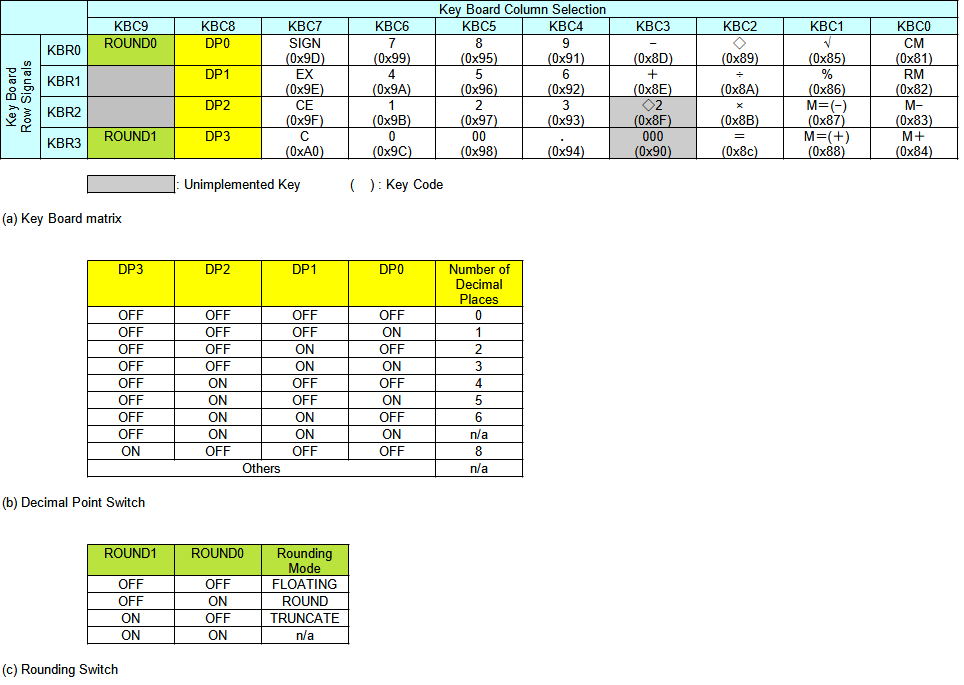
\includegraphics[width=1.00\columnwidth]{./Table/KEYBOARD.png}
    \caption{Keyboard Matrix States and Meanings of the Calculator}
    \label{tb:KEYBOARD}
\end{table}
%----------------------------------

%--------------------------------------------------------------
\subsection{Printing Mechanism of the Calculator}
The calculation results of the 141-PF calculator are printed out via a built-in printer. As previously mentioned, the adopted printer model is the Model 102 from Shinshu Seiki Co. (now Seiko Epson). The internal printing mechanism is illustrated in Figure~\ref{fig:PRINTINGMECHANISM}.

A rotating drum is embedded with convex typesetting characters. Above the drum are layered, in order: paper, ink ribbon, and a hammer. When a desired character on the drum rotates into position beneath the paper, the hammer strikes in precise timing, transferring the ink to the paper via impact. This mechanism is synchronized to ensure accurate printing at each target position.

%----------------------------------
\begin{figure}[htbp]
  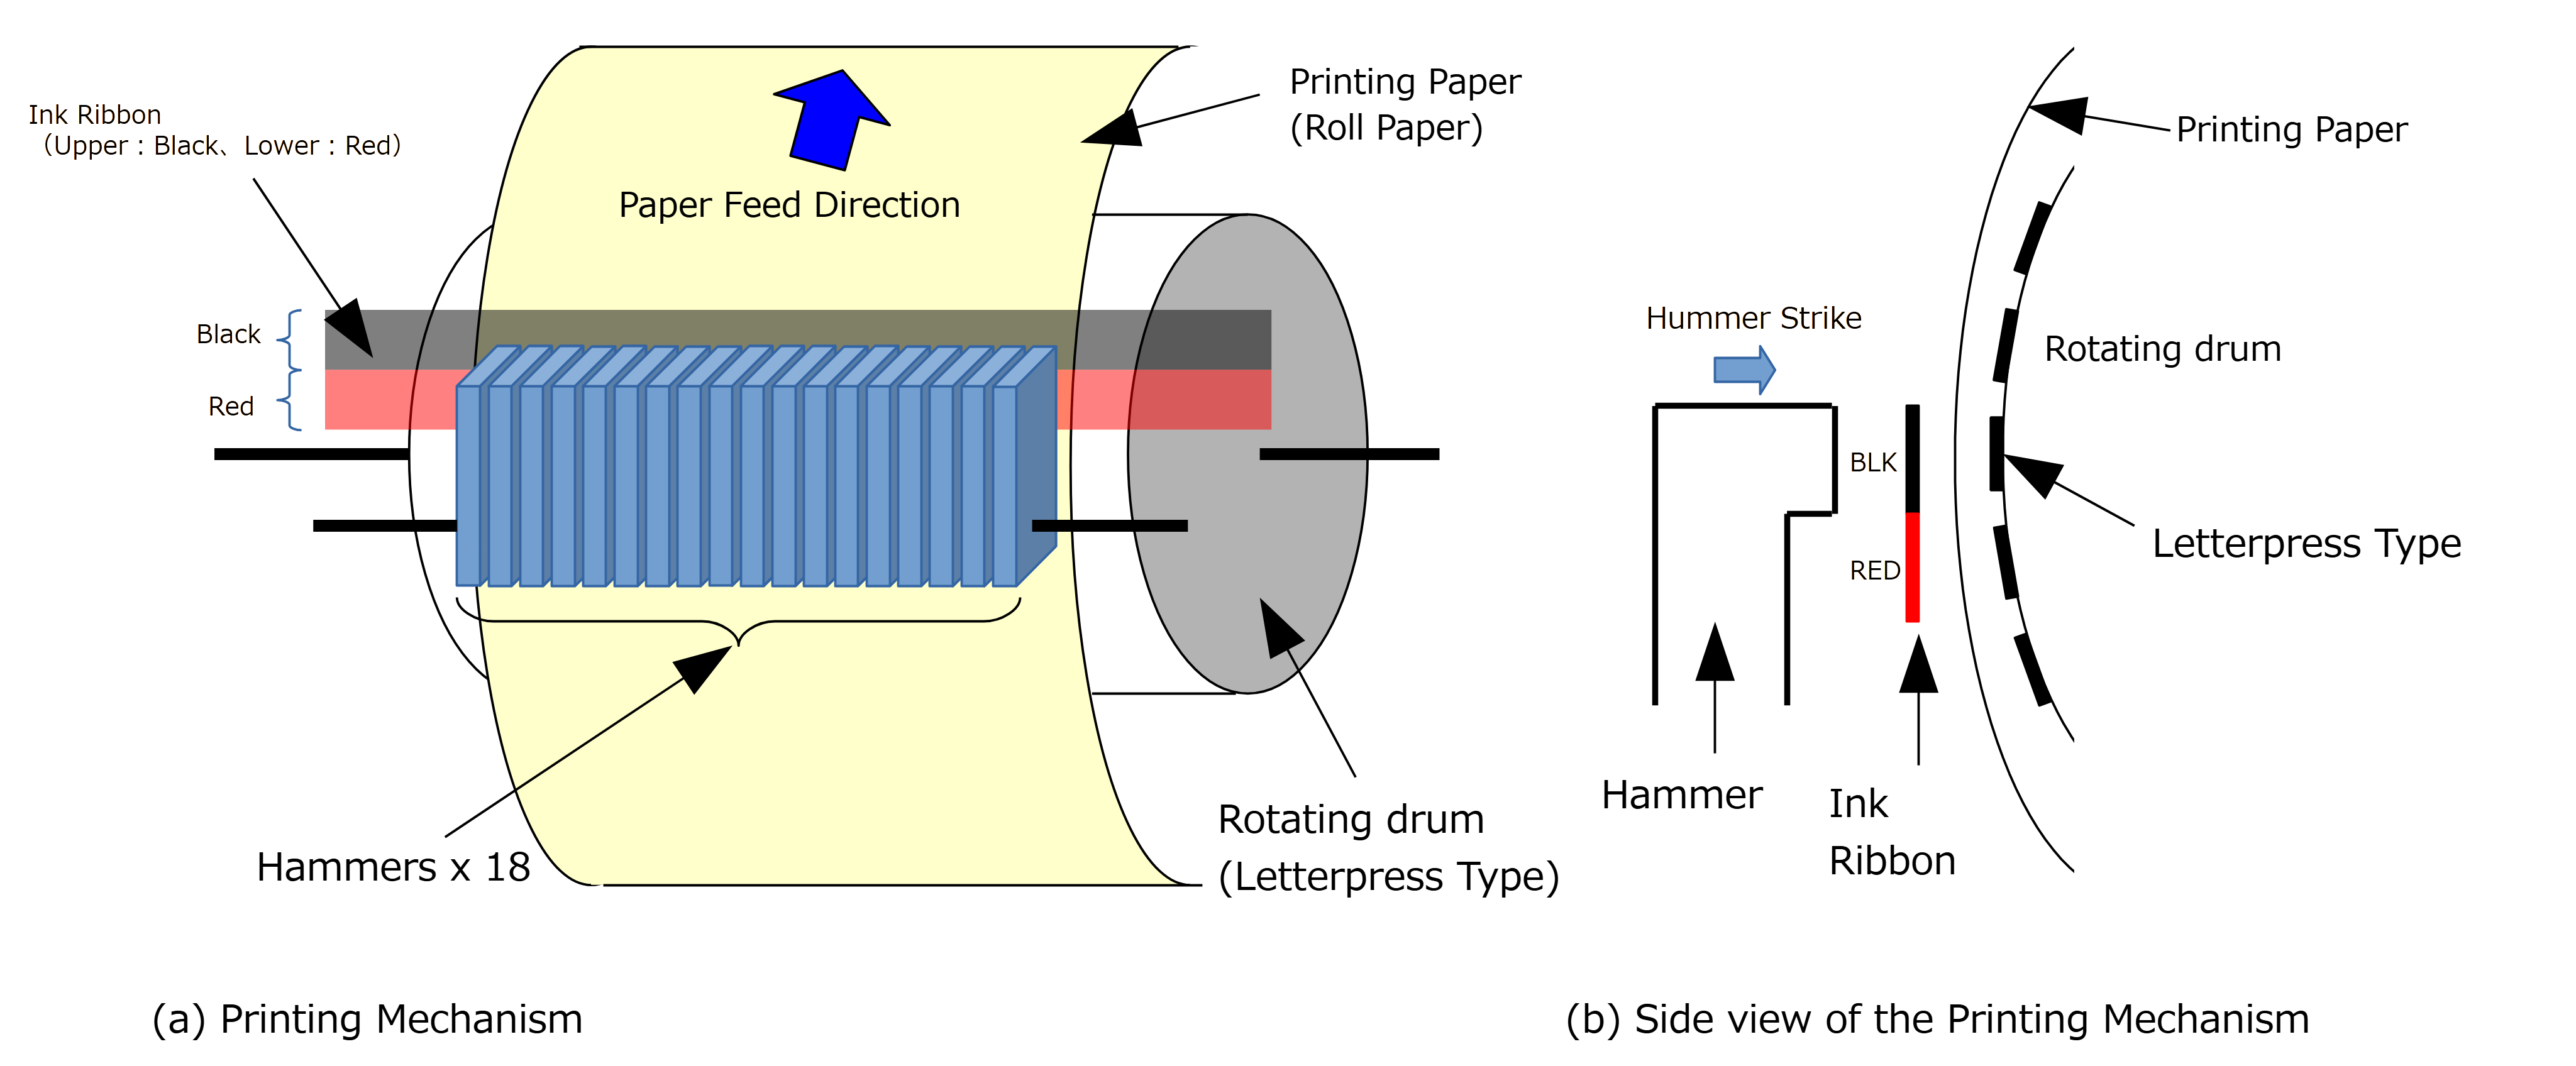
\includegraphics[width=1.0\textwidth]{./Figure/PrintingMechanism.png}
  \caption{Printing Mechanism of the Calculator}
  \label{fig:PRINTINGMECHANISM}
\end{figure}
%----------------------------------

%--------------------------------------------------------------
\subsection{Rotating Drum and Status Signals of the Printer}
The rotating drum of the Busicom 141-PF calculator's printer contains embedded typesetting characters, as illustrated in Table~\ref{tb:PRINTERDRUM}. Conceptually, the drum forms a cylindrical shape where the top and bottom edges of Table~\ref{tb:PRINTERDRUM} connect in a loop.

Horizontally, the drum holds 18 columns (digits), including control characters. However, no type is embedded in Column 16, which always results in a blank space on the printed paper. Vertically, the drum is divided into 13 sectors (rows), each containing a full set of characters.

As the drum rotates, it outputs a status signal \texttt{DRUM\_SECTOR} to indicate that a sector's characters have reached the print position, where the hammer can strike. The 4004 CPU detects this signal via its \texttt{TEST} pin to activate the hammer in precise synchronization.

To determine the rotational position of the drum, a separate signal \texttt{DRUM\_INDEX} is generated when Sector~0's characters align with the print position. This signal is read via IO0 on 4001 (ROM) \#2.

The \texttt{DRUM\_SECTOR} signal is output at approximately 28~ms intervals (frequency = 35.7~Hz), while the \texttt{DRUM\_INDEX} signal occurs once every full rotation of 13 sectors, i.e., every 364~ms (frequency = 2.74~Hz).

%----------------------------------
\begin{table}[htbp]
    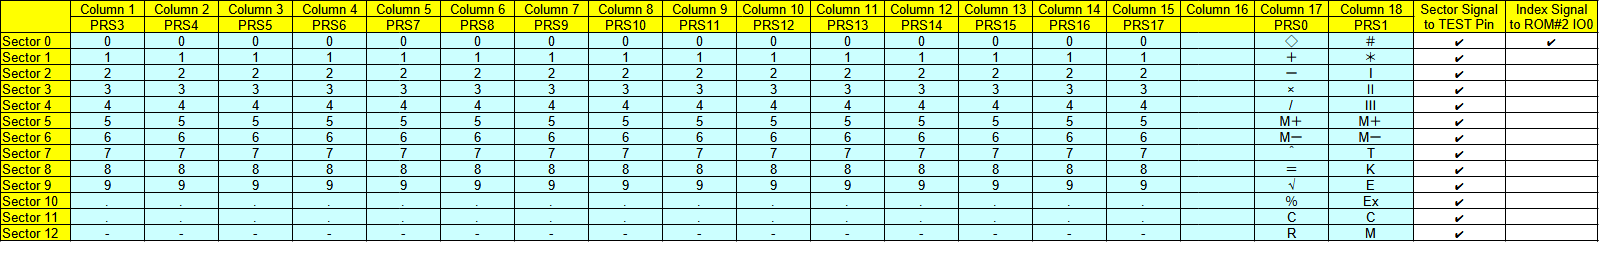
\includegraphics[width=1.00\columnwidth]{./Table/PrinterDrum.png}
    \caption{Rotating Drum of the Printer}
    \label{tb:PRINTERDRUM}
\end{table}
%----------------------------------

%--------------------------------------------------------------
\subsection{Hammer Control of the Printer}
The 141-PF calculator program reads the rotational position of the drum and sequentially issues hammer strike commands for the characters that appear earliest on the drum. There are 18 hammers corresponding to the 18 character columns on the drum.

The selection signals for these hammers are labeled \texttt{PRS00} to \texttt{PRS19}, as shown in Figure~\ref{fig:IOBLOCK141PF}, and are output from 4003 \#1 and 4003 \#2. These shift registers are connected in a cascade configuration. The clock signal is supplied via IO2 of 4001 (ROM) \#0, and shift input data is provided via IO1 of the same ROM. Although the shift input data line is shared with the 4003 \#0 used for the keyboard matrix, the shift clocks are separate, allowing independent operation without conflict.

The correspondence between \texttt{PRS00}–\texttt{PRS19} and actual drum print positions is listed in Table~\ref{tb:PRINTERDRUM}. Note that some signals are unused.

To initiate the hammer strike, the signal \texttt{FIRE\_HAMMERS} is asserted. This signal is output from O1 of 4002 (RAM) \#0. As a result, the hammers selected by \texttt{PRS00}–\texttt{PRS19} are activated simultaneously at the timing of \texttt{FIRE\_HAMMERS}. Multiple hammers may be fired at the same time.

%--------------------------------------------------------------
\subsection{Printing Sequence of the Calculator's Printer}
An example of the printing sequence is shown in Table~\ref{tb:PRINTSEQUENCE}. Here, we consider the case where the string “1.4142135623730 SQ” is printed. Since the 141-PF program continuously monitors the rotational position of the drum, printing can begin from the sector that is approaching the print position first. In this example, Sector~0 is assumed to be next in line for printing.

First, the hammer selection signals (\texttt{PRS00}–\texttt{PRS19}) corresponding to the characters in Sector~0 are configured, and the hammer is triggered. In this case, only Column~15 (character “0”) is activated, since the digit “0” appears only once in the numeric result.

As the drum rotates, Sector~1 approaches the print position. Again, hammer selection signals are configured for the printable characters, and the hammer is triggered. Here, the digit “1” appears three times in the numeric result, so the corresponding hammer signals for those columns are asserted.

This process continues up to Sector~12. As a result, the printed output is not produced sequentially from left to right. Instead, characters across various columns are struck sector-by-sector in a scattered order, and the full result gradually appears once all necessary sectors have passed.

%----------------------------------
\begin{table}[htbp]
    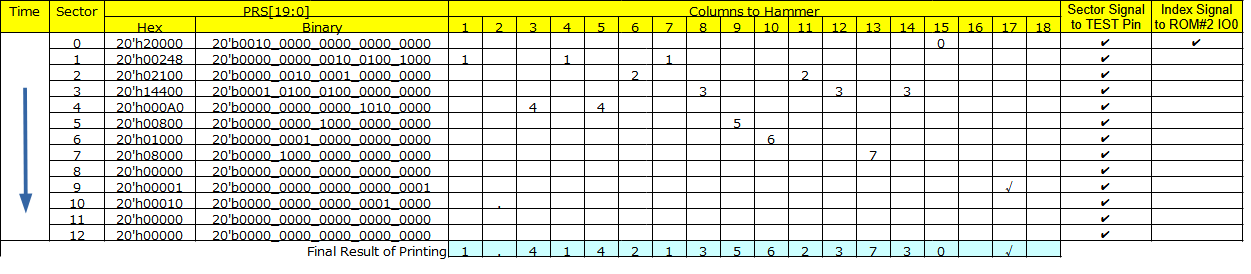
\includegraphics[width=1.00\columnwidth]{./Table/PrintSequence.png}
    \caption{Printing Sequence Example of the Calculator's Printer}
    \label{tb:PRINTSEQUENCE}
\end{table}
%----------------------------------

%--------------------------------------------------------------
\subsection{Ink Ribbon and Paper Feed Control}
Before a character is struck by the hammer, the printing color is specified via the \texttt{PRINTING\_COLOR} signal, which is provided from \texttt{4002(RAM) \#0}, output pin \texttt{O1}. A value of 0 indicates black ink, while a value of 1 selects red ink.

After a full line has been printed, the paper is advanced by asserting the \texttt{ADVANCE\_PAPER} signal from \texttt{4002(RAM) \#0}, output pin \texttt{O3}. This signal is also triggered when the paper feed button is manually pressed.

%--------------------------------------------------------------
\subsection{Paper Feed Button}
The paper feed button is not part of the keyboard matrix. As shown in Figure~\ref{fig:IOBLOCK141PF}, it is connected to \texttt{4001(ROM) \#2} at input/output pin \texttt{IO3}.

%--------------------------------------------------------------
\subsection{Status Indicator Lamps}
Three status indicator lamps are provided to reflect internal conditions:
\begin{itemize}
  \item \textbf{V}: Overflow occurred
  \item \textbf{N}: Result is negative
  \item \textbf{M}: Memory data valid
\end{itemize}
These indicators are controlled via \texttt{4002(RAM) \#1}, output pins \texttt{O0} to \texttt{O2}, respectively.

%--------------------------------------------------------------
\subsection{\texttt{KEY\_PRINTER} Controlled by the RISC-V Subsystem}
The module \texttt{KEY\_PRINTER} implements the logic that emulates the I/O circuitry of the previously described Busicom 141-PF calculator. The RTL description is provided in \texttt{key\_printer.v}. \texttt{KEY\_PRINTER} is controlled via the input/output ports of the RISC-V subsystem. Through coordinated operation between \texttt{KEY\_PRINTER} and the RISC-V subsystem, the I/O behavior of the 141-PF calculator is faithfully reproduced.

Table~\ref{tb:PORTKEYPRTCMD} lists the command signals \texttt{PORT\_KEYPRT\_CMD[31:0]} sent from the RISC-V subsystem to \texttt{KEY\_PRINTER}. Table~\ref{tb:PORTKEYPRTRES} shows the response signals \texttt{PORT\_KEYPRT\_RES[31:0]} returned from \texttt{KEY\_PRINTER} to the RISC-V subsystem.

%----------------------------------
\begin{table}[htbp]
    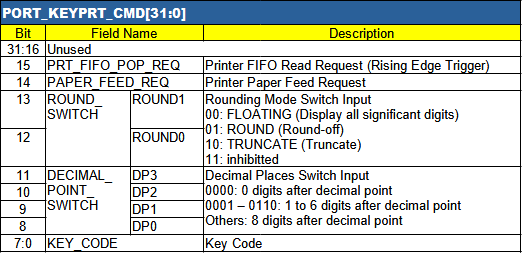
\includegraphics[width=0.75\columnwidth]{./Table/PORTKEYPRTCMD.png}
    \caption{Command Signals Sent to \texttt{KEY\_PRINTER} (Connected to RISC-V Subsystem Ports)}
    \label{tb:PORTKEYPRTCMD}
\end{table}
%----------------------------------
%----------------------------------
\begin{table}[htbp]
    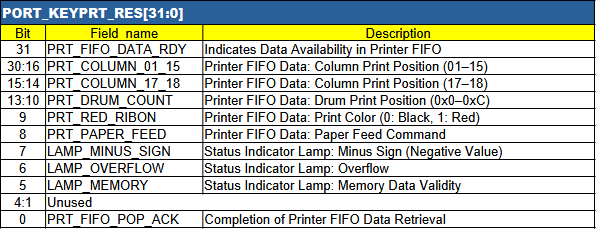
\includegraphics[width=0.75\columnwidth]{./Table/PORTKEYPRTRES.png}
    \caption{Response Signals from \texttt{KEY\_PRINTER} (Connected to RISC-V Subsystem Ports)}
    \label{tb:PORTKEYPRTRES}
\end{table}
%----------------------------------

%--------------------------------------------------------------
\subsection{Keyboard and Switch Emulation}
All control signals related to the keyboard and switches are encapsulated in the command signal described in Table~\ref{tb:PORTKEYPRTCMD}, and are simply passed through to the \texttt{KEY\_PRINTER} module. Upon receiving user interface instructions for key input, the RISC-V subsystem encodes the pressed key type and switch status into specific fields within the lower 15 bits of \texttt{PORT\_KEYPRT\_CMD[31:0]}, which it then outputs. If no key is pressed, the 8-bit \texttt{KEY\_CODE} field is set to \texttt{8'h00}.

In response, \texttt{KEY\_PRINTER} generates the row signals \texttt{KBR0}--\texttt{KBR3} in synchronization with the column scan signals \texttt{KBC0}--\texttt{KBC9}. These signals are then output from \texttt{KEY\_PRINTER}. Additionally, the state of the paper feed button is also output.

%--------------------------------------------------------------
\subsection{Printer Emulation}
When the calculator program for the 141-PF initiates printer operations—such as striking the hammer, advancing the ink ribbon, or feeding paper—the action must be conveyed to the RISC-V subsystem for output to the serial terminal or display on a touch LCD panel.

Due to the complete asynchrony between the 141-PF program and the RISC-V subsystem software, a FIFO buffer with a depth of 256 stages is inserted to store printer operation information. When the 141-PF program performs an action—hammer strike, ribbon movement, or paper feed—the corresponding printer control signals (including drum column position, hammer column selection signals \texttt{PRS00}--\texttt{PRS19}, ink ribbon color selection \texttt{PRINTING\_COLOR}, and paper feed signal \texttt{ADVANCE\_PAPER}) are written into the FIFO.

This information is transmitted to the RISC-V subsystem via the response signal \texttt{PORT\_KEYPRT\_RES[31:0]} (see Table~\ref{tb:PORTKEYPRTRES}). When data is present in the FIFO, bit 15 \texttt{PRT\_FIFO\_DATA\_RDY} is set to 1, indicating that the RISC-V subsystem should read the printer data from bits 8 to 30.

After the RISC-V subsystem reads the data, it asserts bit 15 \texttt{PRT\_FIFO\_POP\_REQ} of \texttt{PORT\_KEYPRT\_CMD[31:0]} to inform \texttt{KEY\_PRINTER} that the FIFO entry was consumed. Upon acknowledgment, \texttt{KEY\_PRINTER} asserts bit 0 \texttt{PRT\_FIFO\_POP\_ACK} of \texttt{PORT\_KEYPRT\_RES[31:0]}, allowing the RISC-V subsystem to clear \texttt{PRT\_FIFO\_POP\_REQ}.

The access procedure for the printer FIFO from the RISC-V subsystem is summarized as follows:

\begin{enumerate}
  \item Periodically monitor \texttt{PORT\_KEYPRT\_RES[31:0]} for \texttt{PRT\_FIFO\_DATA\_RDY} being set.
  \item If set, read printer information from bits 8--30.
  \item Assert \texttt{PRT\_FIFO\_POP\_REQ}.
  \item Wait until \texttt{PRT\_FIFO\_POP\_ACK} is asserted.
  \item Clear \texttt{PRT\_FIFO\_POP\_REQ}.
\end{enumerate}

%--------------------------------------------------------------
\subsection{Emulation of Calculator Status Lamps}
The ON/OFF states of the three calculator status lamps are stored in bits 5 through 7 of the response signal \texttt{PORT\_KEYPRT\_RES[31:0]} from \texttt{KEY\_PRINTER} to the RISC-V subsystem. By periodically monitoring these bits, the RISC-V subsystem reflects the lamp status to the user interface.

%--------------------------------------------------------------
\subsection{Synchronization Across Clock Domains}
The RISC-V subsystem (operating at 20\,MHz) and \texttt{KEY\_PRINTER} (operating at 750\,kHz) function in an asynchronous relationship. Among the command signals sent from the RISC-V subsystem and received by \texttt{KEY\_PRINTER}, key input signals do not undergo synchronization processing, as debounce handling is performed by the 4004 CPU-side software.

However, the \texttt{PRT\_FIFO\_POP\_REQ} signal—used to retrieve printer output data from the FIFO—is synchronized to prevent metastability-induced malfunctions. Response signals from \texttt{KEY\_PRINTER} to the RISC-V subsystem are not synchronized. Nevertheless, during printer FIFO data retrieval, a handshake protocol is followed using \texttt{REQ} (request) and \texttt{ACK} (acknowledge) signals, ensuring stable operation without explicit synchronization logic.

%==============================================================
\section{Program for the 4004 Calculator Model 141-PF}
%--------------------------------------------------------------
\subsection{Program Stored in MCS4\_ROM}
The ROM module of the MCS4\_ROM, which stores programs for the MCS-4 system, is described in RTL reminiscent of SRAM. When synthesized for FPGA, it automatically uses the Block RAM of the FPGA. Since the actual implementation is RAM, the contents are initialized with \verb|$readmemh()| when power is applied to the FPGA at startup. This initialization code is the file \texttt{4001.code}, which is identical to the genuine program code for the Busicom calculator Model 141-PF using MCS-4 chips. The file can be downloaded from \url{http://www.4004.com/assets/busicom-141pf-simulator-w-flowchart-071113.zip}. The system is constructed, including peripheral circuits, to operate this \texttt{4001.code} without any changes.
The license of the code is based on: \\
\url{https://creativecommons.org/licenses/by-nc-sa/2.5/legalcode}

%--------------------------------------------------------------
\subsection{Artistic Program for the 4004 Calculator Model 141-PF}
A detailed explanation of this program's contents, including its disassembly list, is available in the file \texttt{Busicom-141PF-Calculator\_asm\_rel-1-0-1.txt}, which can be downloaded from \url{http://www.4004.com/2009/Busicom-141PF-Calculator_asm_rel-1-0-1.txt}. Reading this file reveals how exceptionally well-designed this program is, making it feel like solving a puzzle. For keyboard matrix input scanning, the program implements features that eliminate chattering while detecting simultaneous presses of keys in the same column, thereby excluding such inputs. Additionally, even while printing results after an operation, the program allows up to 8 stroke inputs for the next keys, enhancing usability.
The license of the disassembly document is based on: \\
\url{https://creativecommons.org/licenses/by-nc-sa/2.5/legalcode}

%--------------------------------------------------------------
\subsection{Optional Square Root Calculations}
Square root calculations are implemented in the 141-PF calculator and also operate in the newly created system. The performance of these calculations is surprisingly fast. The file \texttt{Busicom-141PF-Calculator\_asm\_rel-1-0-1.txt} contains a detailed explanation of the algorithm, which is simply marvelous. Incidentally, this square root calculation was treated as an option for the 141-PF, and most of the actual machines produced at the time lacked square root keys. To add square root calculations, an additional 4001 (ROM) containing the square root program needs to be integrated. 

Apart from square root calculations, the basic calculator program is 1024 bytes (addresses 0x000–0x3FF). The square root program occupies 256 bytes (addresses 0x400–0x4FF). Both are highly compact, with no need for kilobytes or megabytes. 

The program for the 4004 Calculator Model 141-PF is an intricately thought-out masterpiece. It is truly astonishing how all these functions are contained in less than 1280 bytes of code.

%==============================================================
\section{RISC-V Subsystem}
%--------------------------------------------------------------
\subsection{Hardware of the RISC-V Subsystem}
The RISC-V subsystem leverages the SoC system design based on the \texttt{mmRISC-1} core \cite{mmRISC-1}. Detailed information about the design of \texttt{mmRISC-1} and its SoC system can be found at \url{https://github.com/munetomo-maruyama/mmRISC-1}.

The RTL of the built-in RISC-V subsystem is stored under the directory \texttt{RTL/RISCV/}. The top-level description of the RISC-V subsystem is \texttt{RTL/RISCV/riscv\_top/riscv\_top.v}. Debug interface supports only the 4-wire JTAG, with the 2-wire cJTAG support being removed.

The original configuration for GPIO was 32 bits × 3 (GPIO0[31:0]–GPIO2[31:0]). However, this system extends the GPIO to 32 bits × 6 (GPIO0[31:0]–GPIO5[31:0]). Consequently, the \texttt{PORT} module description at \texttt{RTL/RISCV/port/port.v} has been modified. The address mapping for registers in the extended \texttt{PORT} module is shown in Table~\ref{tb:PORTREG}. For GPIO3 to GPIO5, additional registers (\texttt{PDR3}–\texttt{PDR5}, \texttt{PDD3}–\texttt{PDD5}) have been implemented with the same functionalities as those of \texttt{PDR0}–\texttt{PDR2} and \texttt{PDD0}–\texttt{PDD2}.

\begin{table}[h!]
\centering
\begin{tabular}{|l|l|l|}
\hline
\textbf{Offset} & \textbf{Name} & \textbf{Description} \\ \hline
0x00            & PDR0          & Port Data Register 0 \\ \hline
0x04            & PDR1          & Port Data Register 1 \\ \hline
0x08            & PDR2          & Port Data Register 2 \\ \hline
0x0c            & PDR3          & Port Data Register 3 \\ \hline
0x10            & PDR4          & Port Data Register 4 \\ \hline
0x14            & PDR5          & Port Data Register 5 \\ \hline
0x20            & PDD0          & Port Data Direction 0 \\ \hline
0x24            & PDD1          & Port Data Direction 1 \\ \hline
0x28            & PDD2          & Port Data Direction 2 \\ \hline
0x2c            & PDD3          & Port Data Direction 3 \\ \hline
0x30            & PDD4          & Port Data Direction 4 \\ \hline
0x34            & PDD5          & Port Data Direction 5 \\ \hline
\end{tabular}
\caption{Registers in the PORT Module}
\label{tb:PORTREG}
\end{table}

Among the ports, GPIO0 to GPIO2 are routed externally from the FPGA, as shown in Tables~\ref{tb:EXTGPIO0}, \ref{tb:EXTGPIO1}, and \ref{tb:EXTGPIO2}. Meanwhile, GPIO3 to GPIO5 are connected internally within the FPGA, as detailed in Tables~\ref{tb:INTGPIO3}, \ref{tb:INTGPIO4}, and \ref{tb:INTGPIO5}.

%----------------------------------
\begin{table}
    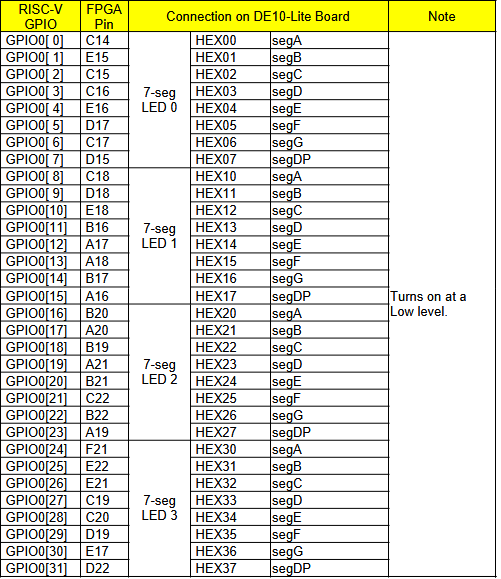
\includegraphics[width=0.5\columnwidth]{./Table/EXTGPIO0.png}
    \caption{GPIO0 connected to External Pins}
    \label{tb:EXTGPIO0}
\end{table}
%----------------------------------
%----------------------------------
\begin{table}
    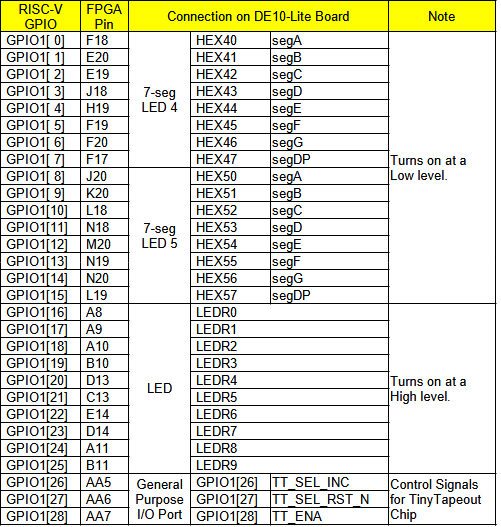
\includegraphics[width=0.5\columnwidth]{./Table/EXTGPIO1.png}
    \caption{GPIO1 connected to External Pins}
    \label{tb:EXTGPIO1}
\end{table}
%----------------------------------
%----------------------------------
\begin{table}
    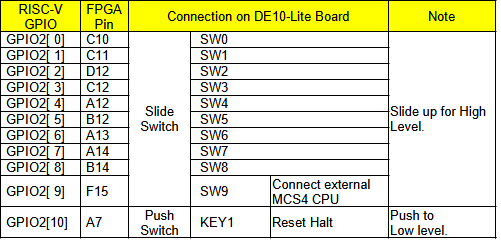
\includegraphics[width=0.5\columnwidth]{./Table/EXTGPIO2.png}
    \caption{GPIO2 connected to External Pins}
    \label{tb:EXTGPIO2}
\end{table}
%----------------------------------
%----------------------------------
\begin{table}
    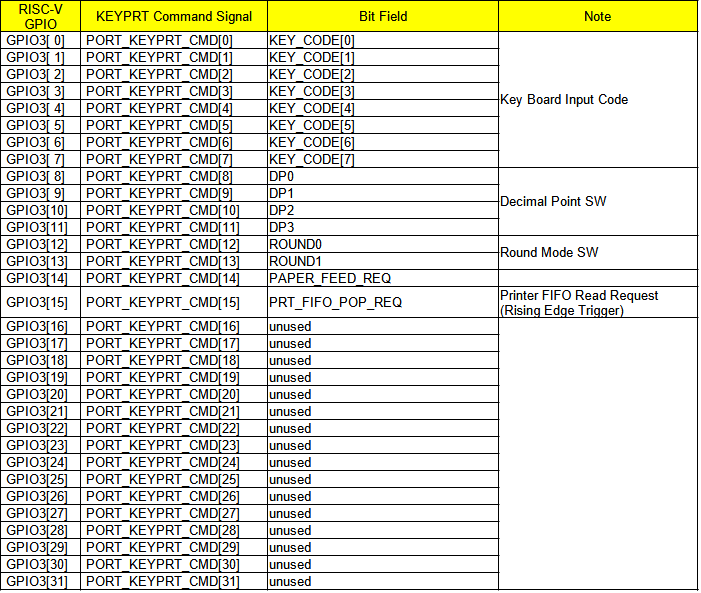
\includegraphics[width=0.75\columnwidth]{./Table/INTGPIO3.png}
    \caption{GPIO3 connected to Internal Signals}
    \label{tb:INTGPIO3}
\end{table}
%----------------------------------
%----------------------------------
\begin{table}
    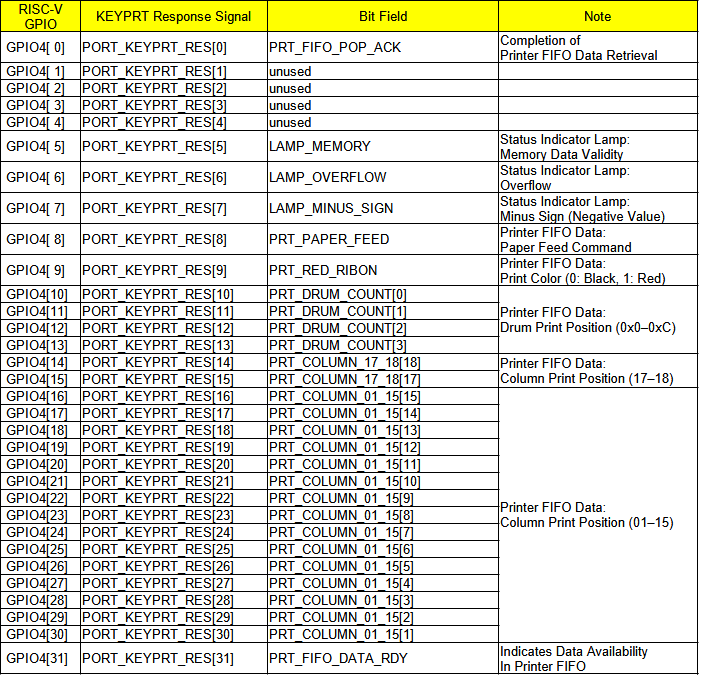
\includegraphics[width=0.75\columnwidth]{./Table/INTGPIO4.png}
    \caption{GPIO4 connected to Internal Signals}
    \label{tb:INTGPIO4}
\end{table}
%----------------------------------
%----------------------------------
\begin{table}
    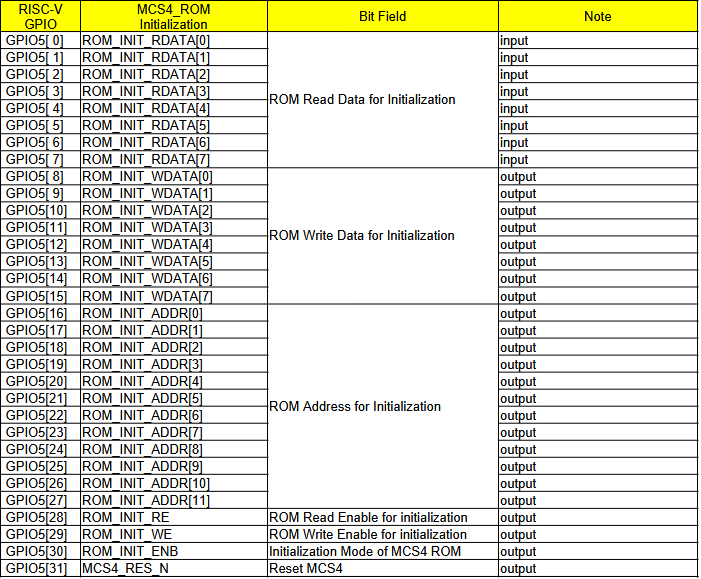
\includegraphics[width=0.75\columnwidth]{./Table/INTGPIO5.png}
    \caption{GPIO5 connected to Internal Signals}
    \label{tb:INTGPIO5}
\end{table}
%----------------------------------

%--------------------------------------------------------------
\subsection{Software of the RISC-V Subsystem}
The software for the RISC-V subsystem was developed using a GCC-based environment within the integrated development environment \texttt{Eclipse Embedded CDT}. The workspace and source code are stored in the directory \texttt{SOFTWARE/workspace/MCS4\_141PF}.\\

After startup, the main routine (\texttt{main.c}) determines the presence and type of the touch LCD panel (capacitive or resistive). If the touch LCD panel is not connected, subsequent operations are conducted through the serial terminal. The serial terminal should be configured to \texttt{115200bps}, 8N1 format. When the serial terminal is selected as the user interface, control is handed over to the routines in \texttt{src\_app/src/cui\_141pf.c}.\\

If the touch LCD panel is connected, control is passed to the routines in \texttt{src\_app/src/gui\_141pf.c}, enabling graphical calculator operations through touch interaction.\\

On the DE10-Lite board, resetting with \texttt{SW8 (GPIO2[8])} in the OFF (Low level) state runs the calculator program for the Model 141-PF. When \texttt{SW8} is ON (High level) during reset, the program for 500-digit pi calculation, which will be explained later, is loaded and executed in the \texttt{MCS4\_ROM} module. Switching \texttt{SW8} back to OFF and resetting will reload the 141-PF calculator program into the \texttt{MCS4\_ROM} module for execution.\\

The 500-digit pi calculation program solely prints the results. Even if the touch LCD panel is connected, the calculation results are displayed on the serial terminal.\\

The software for the RISC-V subsystem is constructed to run on the FreeRTOS for RISC-V ported by the author for \texttt{mmRISC-1}. The RTOS kernel is stored in \texttt{src/src\_kernel}, while the applications are stored in \texttt{src/src\_app}. In the calculator control routines (\texttt{src\_app/src/cui\_141pf.c} and \texttt{src\_app/src/gui\_141pf.c}), tasks for keyboard control and printer control operate independently. Furthermore, in \texttt{src\_app/src/cui\_141pf.c}, using the serial terminal, a semaphore notifies the keyboard control task whenever the UART receives a character, triggered by its interrupt service routine.

%--------------------------------------------------------------
\subsection{When Modifying Software of the RISC-V Subsystem}
The binary software of the RISC-V subsystem initializes the memory components (\texttt{s\_mem0} to \texttt{s\_mem3}) within the instruction memory (\texttt{RISCV/ram/rami.v}) using the \verb|$readmemh| command. Each memory component is byte-wide, and their respective initialization files are \texttt{MCS4\_141PF.rom0} to \texttt{MCS4\_141PF.rom3}. These files are created by converting the Intel Hex binary \texttt{SOFTWARE/workspace/MCS4\_141PF/debug/MCS4\_141PF.hex} of the program. The conversion tools are located in the \texttt{SOFTWARE/tools} directory: \texttt{hex2v32\_lane0.exe} to \texttt{hex2v32\_lane3.exe}. These tools are built using source files written in standard C (\texttt{hex2v32\_lane0.c} to \texttt{hex2v32\_lane3.c}).

Once the four conversion tools are prepared, navigate to the directory \texttt{RTL/RISCV/ram} and execute the shell script below to generate the initialization files for \verb|$readmemh|:

\begin{verbatim}
$ ./gen_init
\end{verbatim}

Therefore, whenever modifying the \texttt{SOFTWARE/workspace/MCS4\_141PF}, ensure to update the initial values of the instruction memory by running the command above. Subsequently, synthesize the FPGA, and the updated program will operate starting from power-on. The changes will also reflect in the logic simulation described later.

%==============================================================
\section{Logical Simulation of the MCS-4 System}
%--------------------------------------------------------------
\subsection{Logical Simulation of the MCS-4 System Using Icarus Verilog}
The MCS-4 system was simulated separately using Icarus Verilog, while the entire setup including FPGA macro elements and the RISC-V subsystem was simulated using Questa Altera FPGA Starter Edition. This section details the simulation process for the MCS-4 system.

%--------------------------------------------------------------
\subsection{Resources for Simulation}
Resources required for logical simulation with Icarus Verilog are located under the directory \texttt{SIM\_iverilog}. Descriptions in this section assume this directory as the working directory.

%--------------------------------------------------------------
\subsection{Installing Icarus Verilog}
Install Icarus Verilog according to your environment by referring to online information. Also, install the waveform viewer \texttt{gtkwave} for reviewing simulation results.

%--------------------------------------------------------------
\subsection{For Simulation Using 141-PF Calculator Program}
The RTL description of the \texttt{MCS4\_ROM} module initializes the ROM memory with \texttt{4001.code}. Without modification, you can perform the logical simulation using this setup.

%--------------------------------------------------------------
\subsection{For Simulation Using Custom 4004 Program Code}
To simulate using your custom 4004 (CPU) program code:
\begin{enumerate}
    \item Assemble the source program (\texttt{.src}) using the assembler tool ADS4004 to generate the Intel Hex format binary file (\texttt{.hex}).
    \item Convert this file to a Verilog HDL initialization file using the \texttt{hex2v} tool, whose C source is located at \texttt{../SOFTWARE/tools/hex2v.c}.
    \item For example:
    \begin{verbatim}
    $ ../SOFTWARE/tools/hex2v.exe ../SOFTWARE/ADS4004/test.src.hex > ../RTL/MCS4/test.src.hex.code
    \end{verbatim}
    \item Modify the RTL description of \texttt{MCS4\_ROM} (\texttt{../RTL/MCS4/mcs4\_rom.v}) as follows:
    \begin{verbatim}
    $readmemh("../RTL/MCS4/test.src.hex.code", rom);
    \end{verbatim}
\end{enumerate}

The preparation of the 4004 (CPU) program is now complete.

%--------------------------------------------------------------
\subsection{Testbench for 141-PF calculator}
The top-level testbench for logical simulation is \texttt{tb\_TOP.v}. The testbench is designed to verify the operation of the 141-PF calculator by directly manipulating \texttt{PORT\_KEYPRT\_CMD[31:0]} and \texttt{PORT\_KEYPRT\_RES[31:0]} stimuli to simulate keyboard inputs and retrieve printer data. For logical verification with custom 4004 (CPU) program codes, please modify the testbench as necessary.

%--------------------------------------------------------------
\subsection{Execution of the Simulation}
All RTL descriptions required for logical simulation are listed in the file \texttt{flist}. The execution steps for the logical simulation have been compiled into the shell script \texttt{run\_iverilog}. You can execute the script as follows:

\begin{verbatim}
$ ./run_iverilog
\end{verbatim}

The RTL descriptions will be compiled by the \texttt{iverilog} command, and if no errors occur, the executable file \texttt{tb.vvp} is produced. This file is then passed to the main logic simulator \texttt{vvp}, which executes the logical simulation and generates the waveform file \texttt{tb.vcd}.

%--------------------------------------------------------------
\subsection{Viewing Waveform Files}
View the resulting waveform file (\texttt{tb.vcd}) using \texttt{gtkwave}:
\begin{verbatim}
$ gtkwave.exe tb.vcd tb.gtkw
\end{verbatim}

The second argument specified as \texttt{tb.gtkw} is a configuration file for the waveform viewer. This file allows you to freely select display waveforms and specify their order as desired. After arranging the waveform display methods on the viewer and saving the configuration, you can view the waveforms with the same display settings in subsequent sessions as shown in Figure~\ref{fig:WAVE141PF}.

%----------------------------------
\begin{figure}[htbp]
  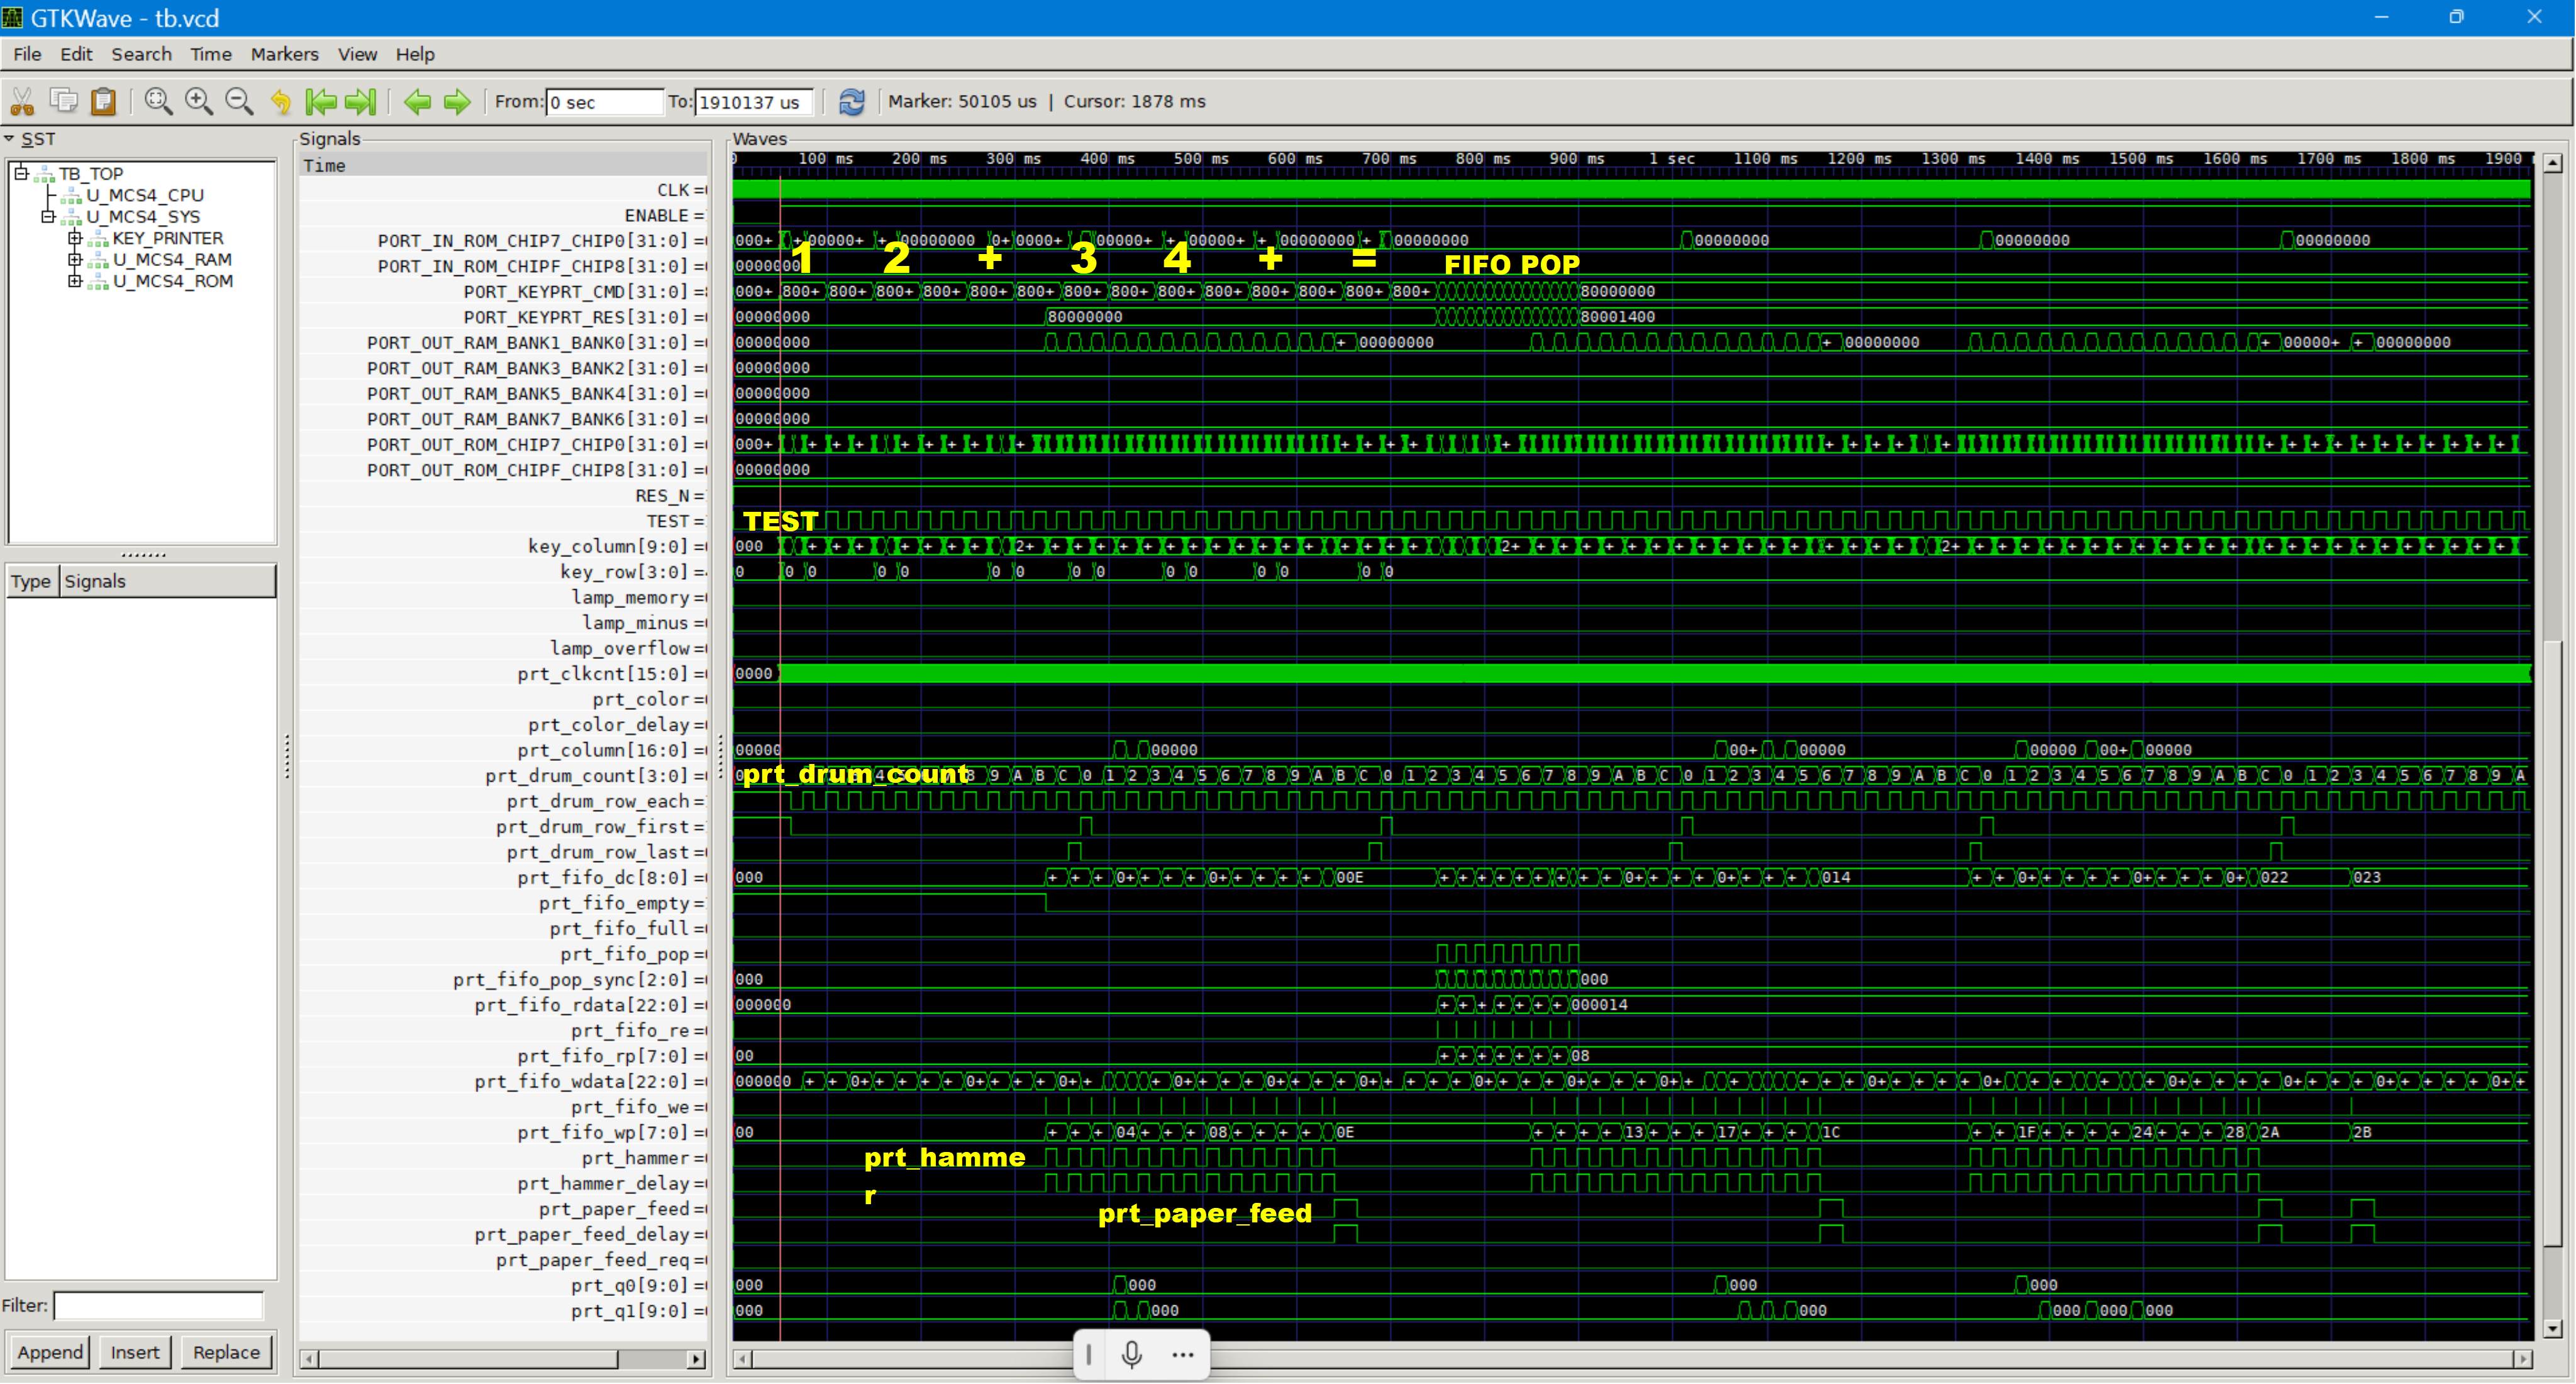
\includegraphics[width=1.0\textwidth]{./Figure/WAVE141PF.png}
  \caption{Waveform of 141-PF Simulation}
  \label{fig:WAVE141PF}
\end{figure}
%----------------------------------


%==============================================================
\section{Logical Simulation of the Entire FPGA System}
%--------------------------------------------------------------
\subsection{Logical Simulation of the Entire FPGA System Using Questa}
The entire FPGA system, including FPGA macro elements and the RISC-V subsystem, is simulated using Questa Altera FPGA Starter Edition. Related resources for Questa-based simulation are stored under the directory \texttt{SIM\_questa}. The following explanation assumes this directory as the working directory.

%--------------------------------------------------------------
\subsection{Executing Logical Simulation Using Questa}
To start Questa, execute the following command:

\begin{verbatim}
$ vsim.exe
\end{verbatim}

Then, within the Transcript window of Questa, execute:

\begin{verbatim}
Questa> do sim_TOP.do
\end{verbatim}

Here, the file \texttt{sim\_TOP.do}, specified as an argument for the \texttt{do} command, is a TCL script that includes the RTL descriptions used for simulation, simulation commands, and waveform display settings. You can modify the waveform display settings and other details as desired. An example of Questa simulation is shown in Figure~\ref{fig:WAVEFPGA}.

%----------------------------------
\begin{figure}[htbp]
  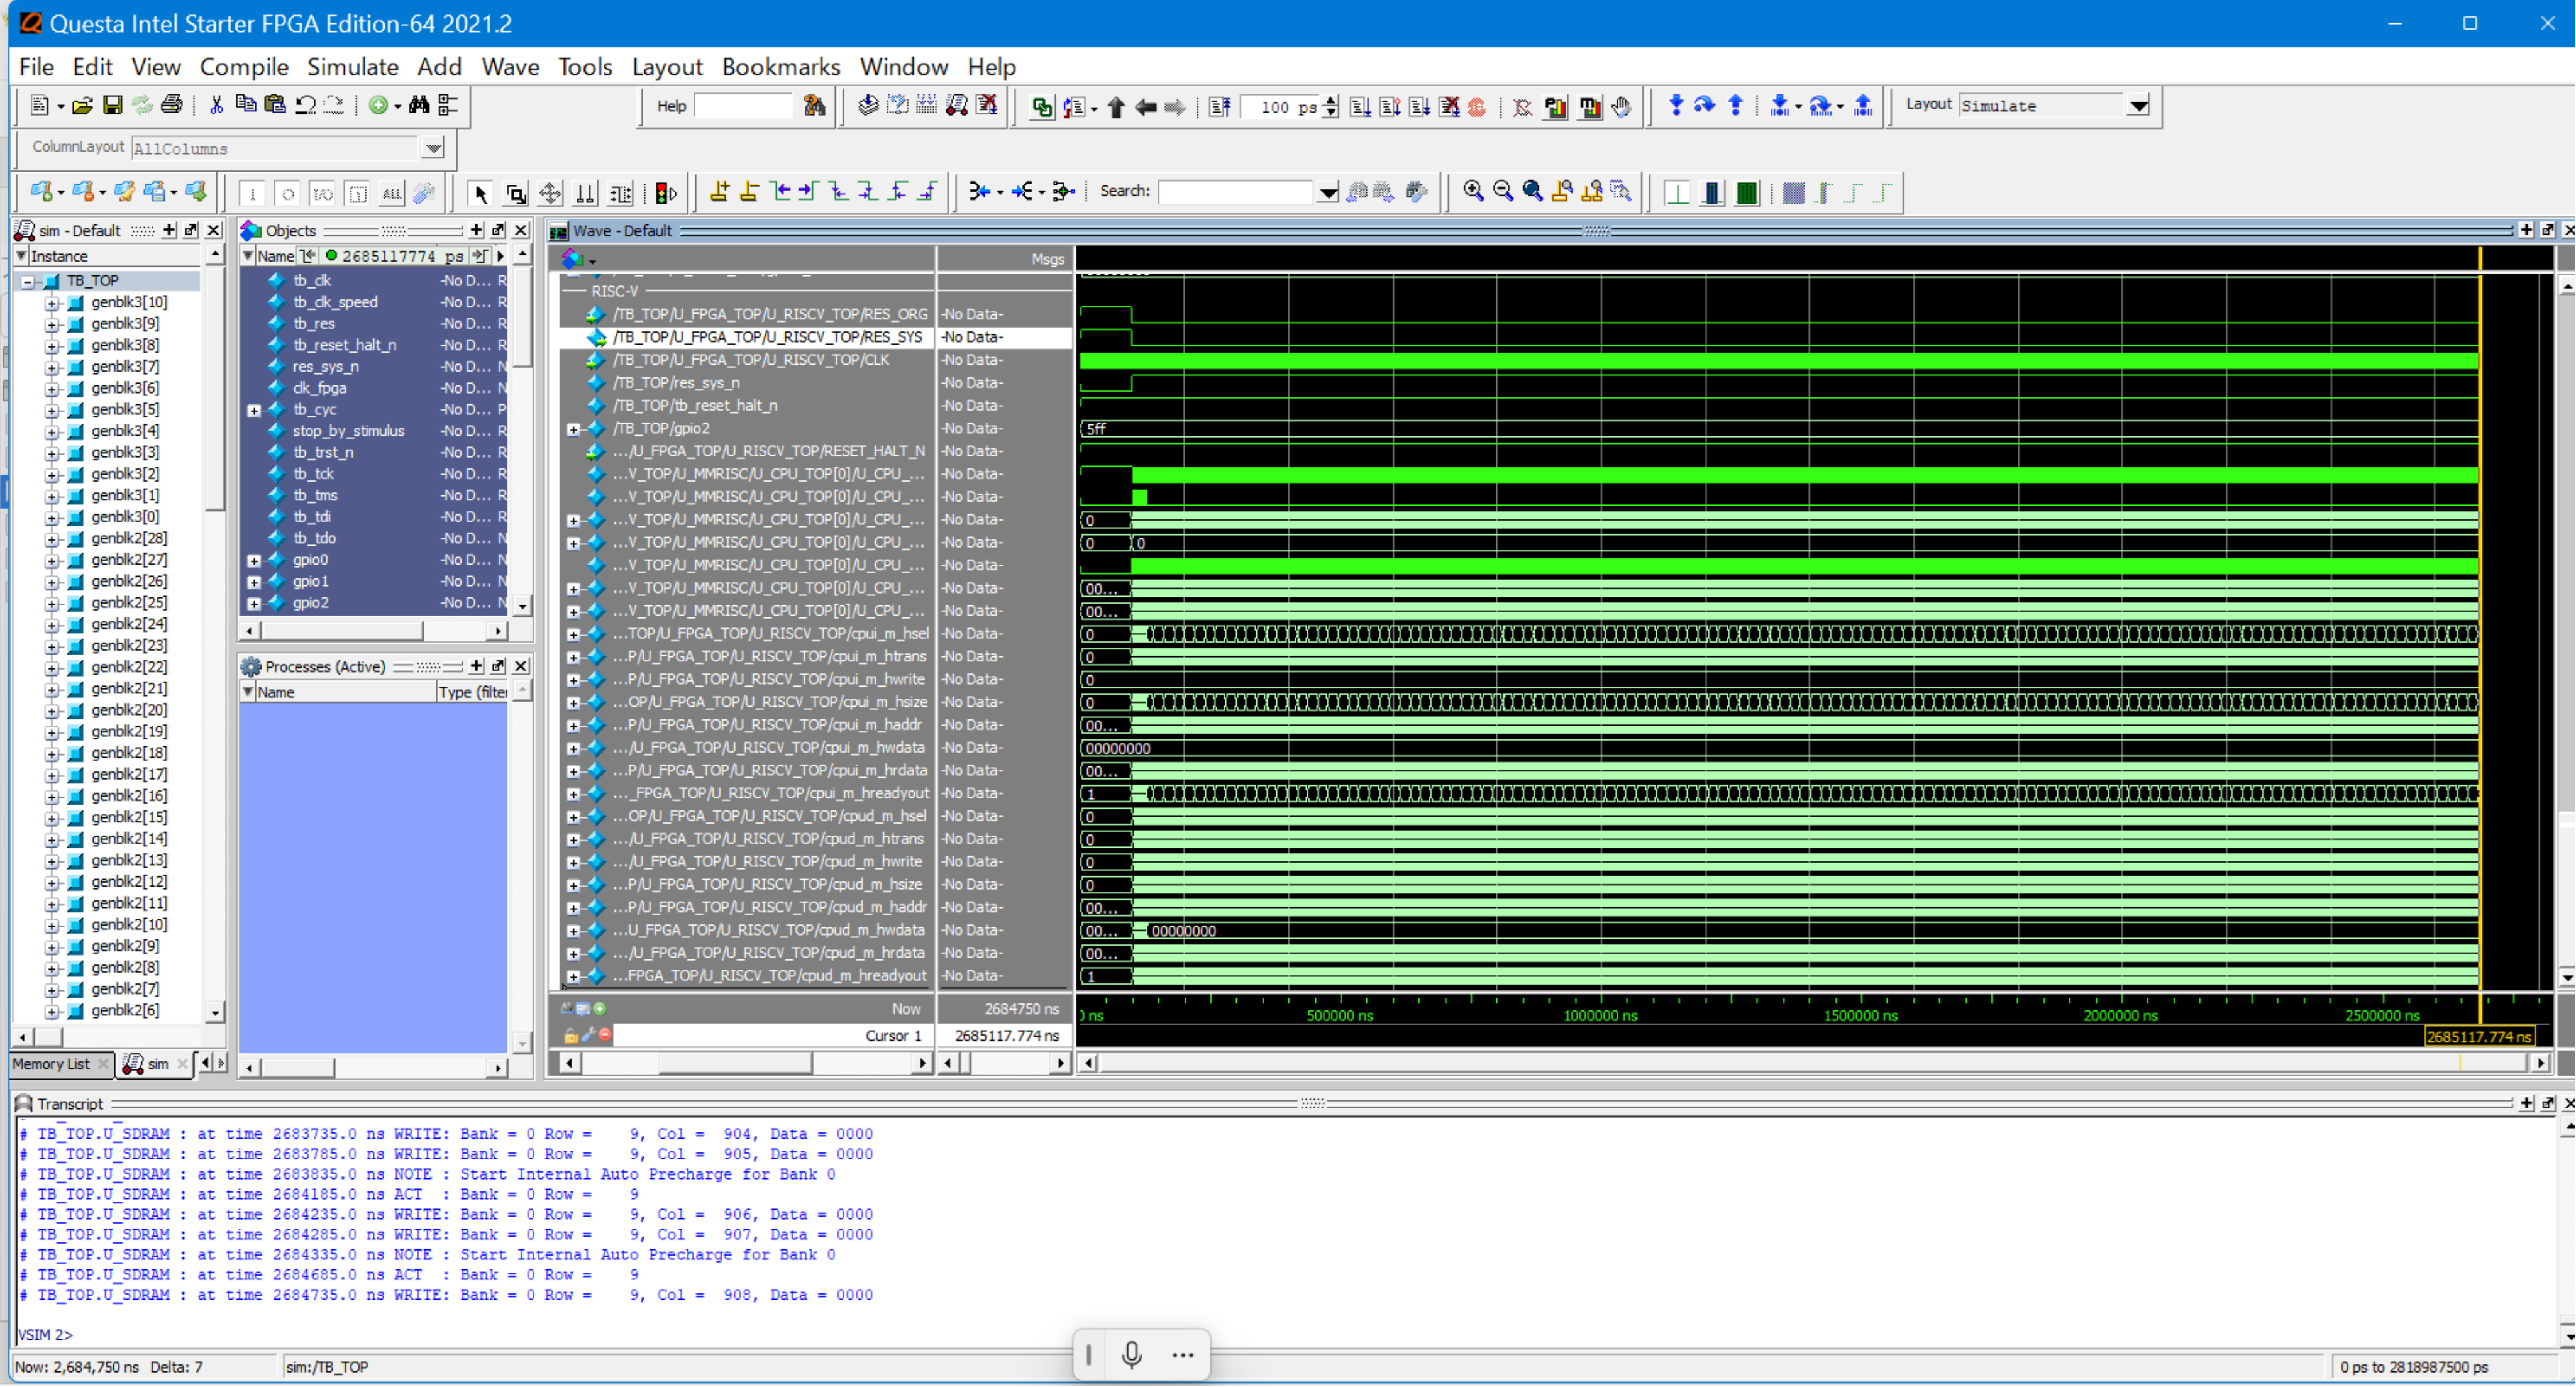
\includegraphics[width=1.0\textwidth]{./Figure/WAVEFPGA.png}
  \caption{Waveform of FPGA Simulation}
  \label{fig:WAVEFPGA}
\end{figure}
%----------------------------------

In this logical simulation, the RISC-V instruction memory \texttt{../RTL/RISCV/ram/rami.v} is initialized using \texttt{../SOFTWARE/workspace/MCS4\_141PF/Debug/MCS4\_141PF.hex}. Since the execution of this program takes time, the purpose of this simulation is primarily to verify the absence of errors in the RTL description, including the top-level FPGA hierarchy. For a detailed inspection of the RISC-V subsystem's operation, it is recommended to replace the RISC-V program with a simpler one and re-execute the simulation.

%==============================================================
\section{FPGA Implementation}
The implementation of Altera FPGA MAX 10 is conducted using the Quartus Prime tool. FPGA-related resources are stored in the directory \texttt{FPGA/}.

%--------------------------------------------------------------
\subsection*{Steps for Synthesis and Configuration}
\begin{enumerate}
    \item Open the Quartus Prime project file located at \texttt{FPGA/FPGA.qpf}.
    \item Perform the synthesis process.
    \item After a successful synthesis without any errors, generate the configuration file (\texttt{FPGA/output\_files/FPGA.pof}).
    \item Use the Quartus Prime tool ``Programmer'' to write the configuration file to the FPGA.
\end{enumerate}

%--------------------------------------------------------------
\subsection{Signal Assignments for External FPGA Terminals}
For the RISC-V subsystem's external terminal assignments related to GPIOs, please refer to Tables~\ref{EXTGPIO0}--\ref{EXTGPIO2}. The assignments for other RISC-V-related external terminals are detailed in Table~\ref{tb:EXTFPGARISCV}.

Within the MCS-4 system, the MCS4\_CPU (4004 CPU) has a mode available for external connection. The signal assignments for this external connection can be found in Table~\ref{tb:EXTFPGAMCS4CPU}.

%----------------------------------
\begin{table}[htbp]
    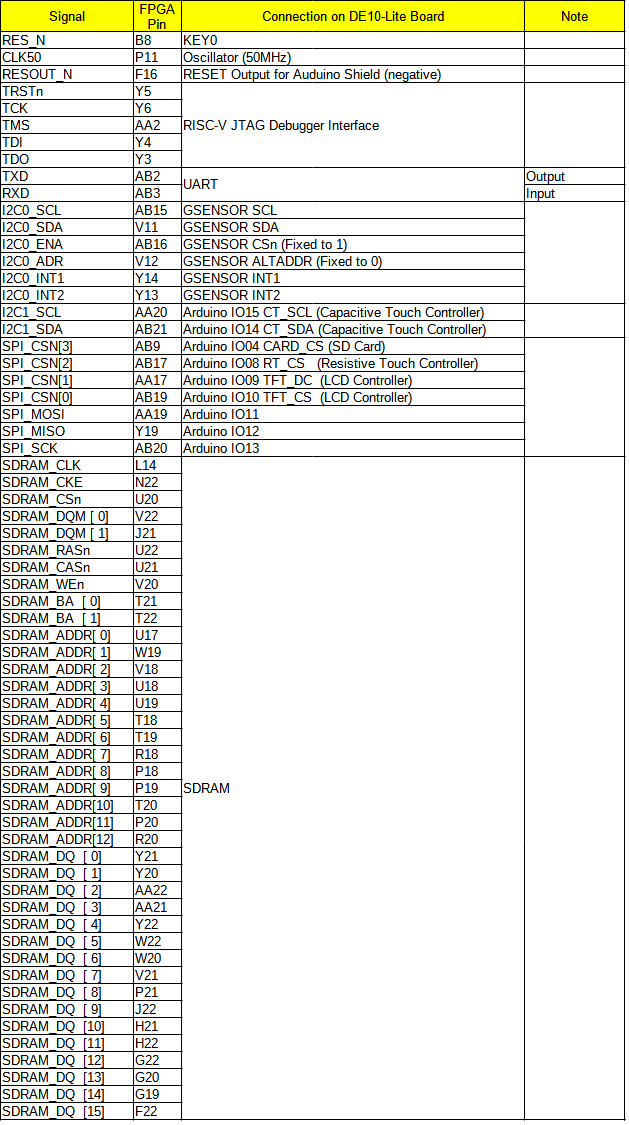
\includegraphics[width=0.5\columnwidth]{./Table/EXTFPGARISCV.png}
    \caption{RISC-V related External Signals except for GPIO}
    \label{tb:EXTFPGARISCV}
\end{table}
%----------------------------------
%----------------------------------
\begin{table}[htbp]
    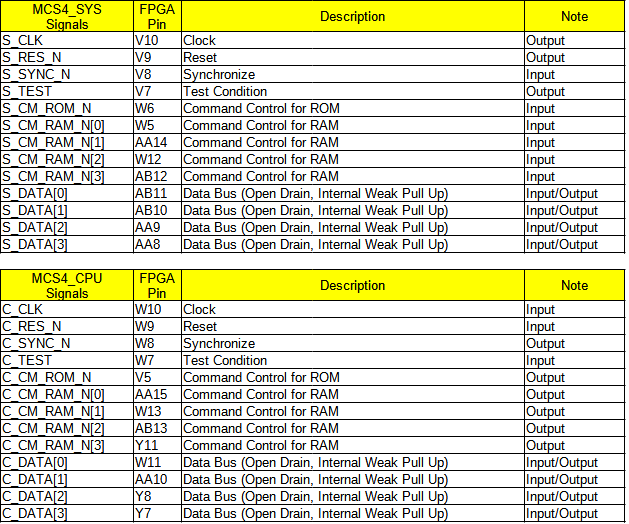
\includegraphics[width=0.5\columnwidth]{./Table/EXTFPGAMCS4CPU.png}
    \caption{MCS4\_CPU (4004 CPU) related External Signals}
    \label{tb:EXTFPGAMCS4CPU}
\end{table}
%----------------------------------

%--------------------------------------------------------------
\subsection{MCS4\_CPU Connection Methods and DE10-Lite Board Settings}
\paragraph{Case A:} When the MCS4\_CPU (4004 CPU) is connected and operated within the FPGA, the DE10-Lite board settings are shown in Figure~\ref{fig:FPGACASEA}. There are no external connections related to the MCS4\_CPU (4004 CPU). In this mode, set the slide switch SW9 to OFF.

\paragraph{Case B:} When using the internal logic of the MCS4\_CPU (4004 CPU) in the FPGA but connecting through external terminals, the DE10-Lite board settings are shown in Figure~\ref{fig:FPGACASEB}. Connect the MCS4\_CPU (4004 CPU) with the MCS4\_SYS via external connectors. As indicated by the red lines, connect the opposing terminals. In this mode, set the slide switch SW9 to ON.

\paragraph{Case C:} When connecting an external device with equivalent functionality to the MCS4\_CPU (4004 CPU) via external terminals, the DE10-Lite board settings are shown in Figure~\ref{fig:FPGACASEC}. Connect the external device's MCS4\_CPU (4004 CPU) to the terminals on the MCS4\_SYS side. In this mode, set the slide switch SW9 to ON.

For all cases above, the UART communication signals (TXD, RXD) should be connected to terminal software on a PC (115200bps, 8N1) via a USB-UART conversion board or the USB-JTAG interface board described later.

%----------------------------------
\begin{figure}[htbp]
  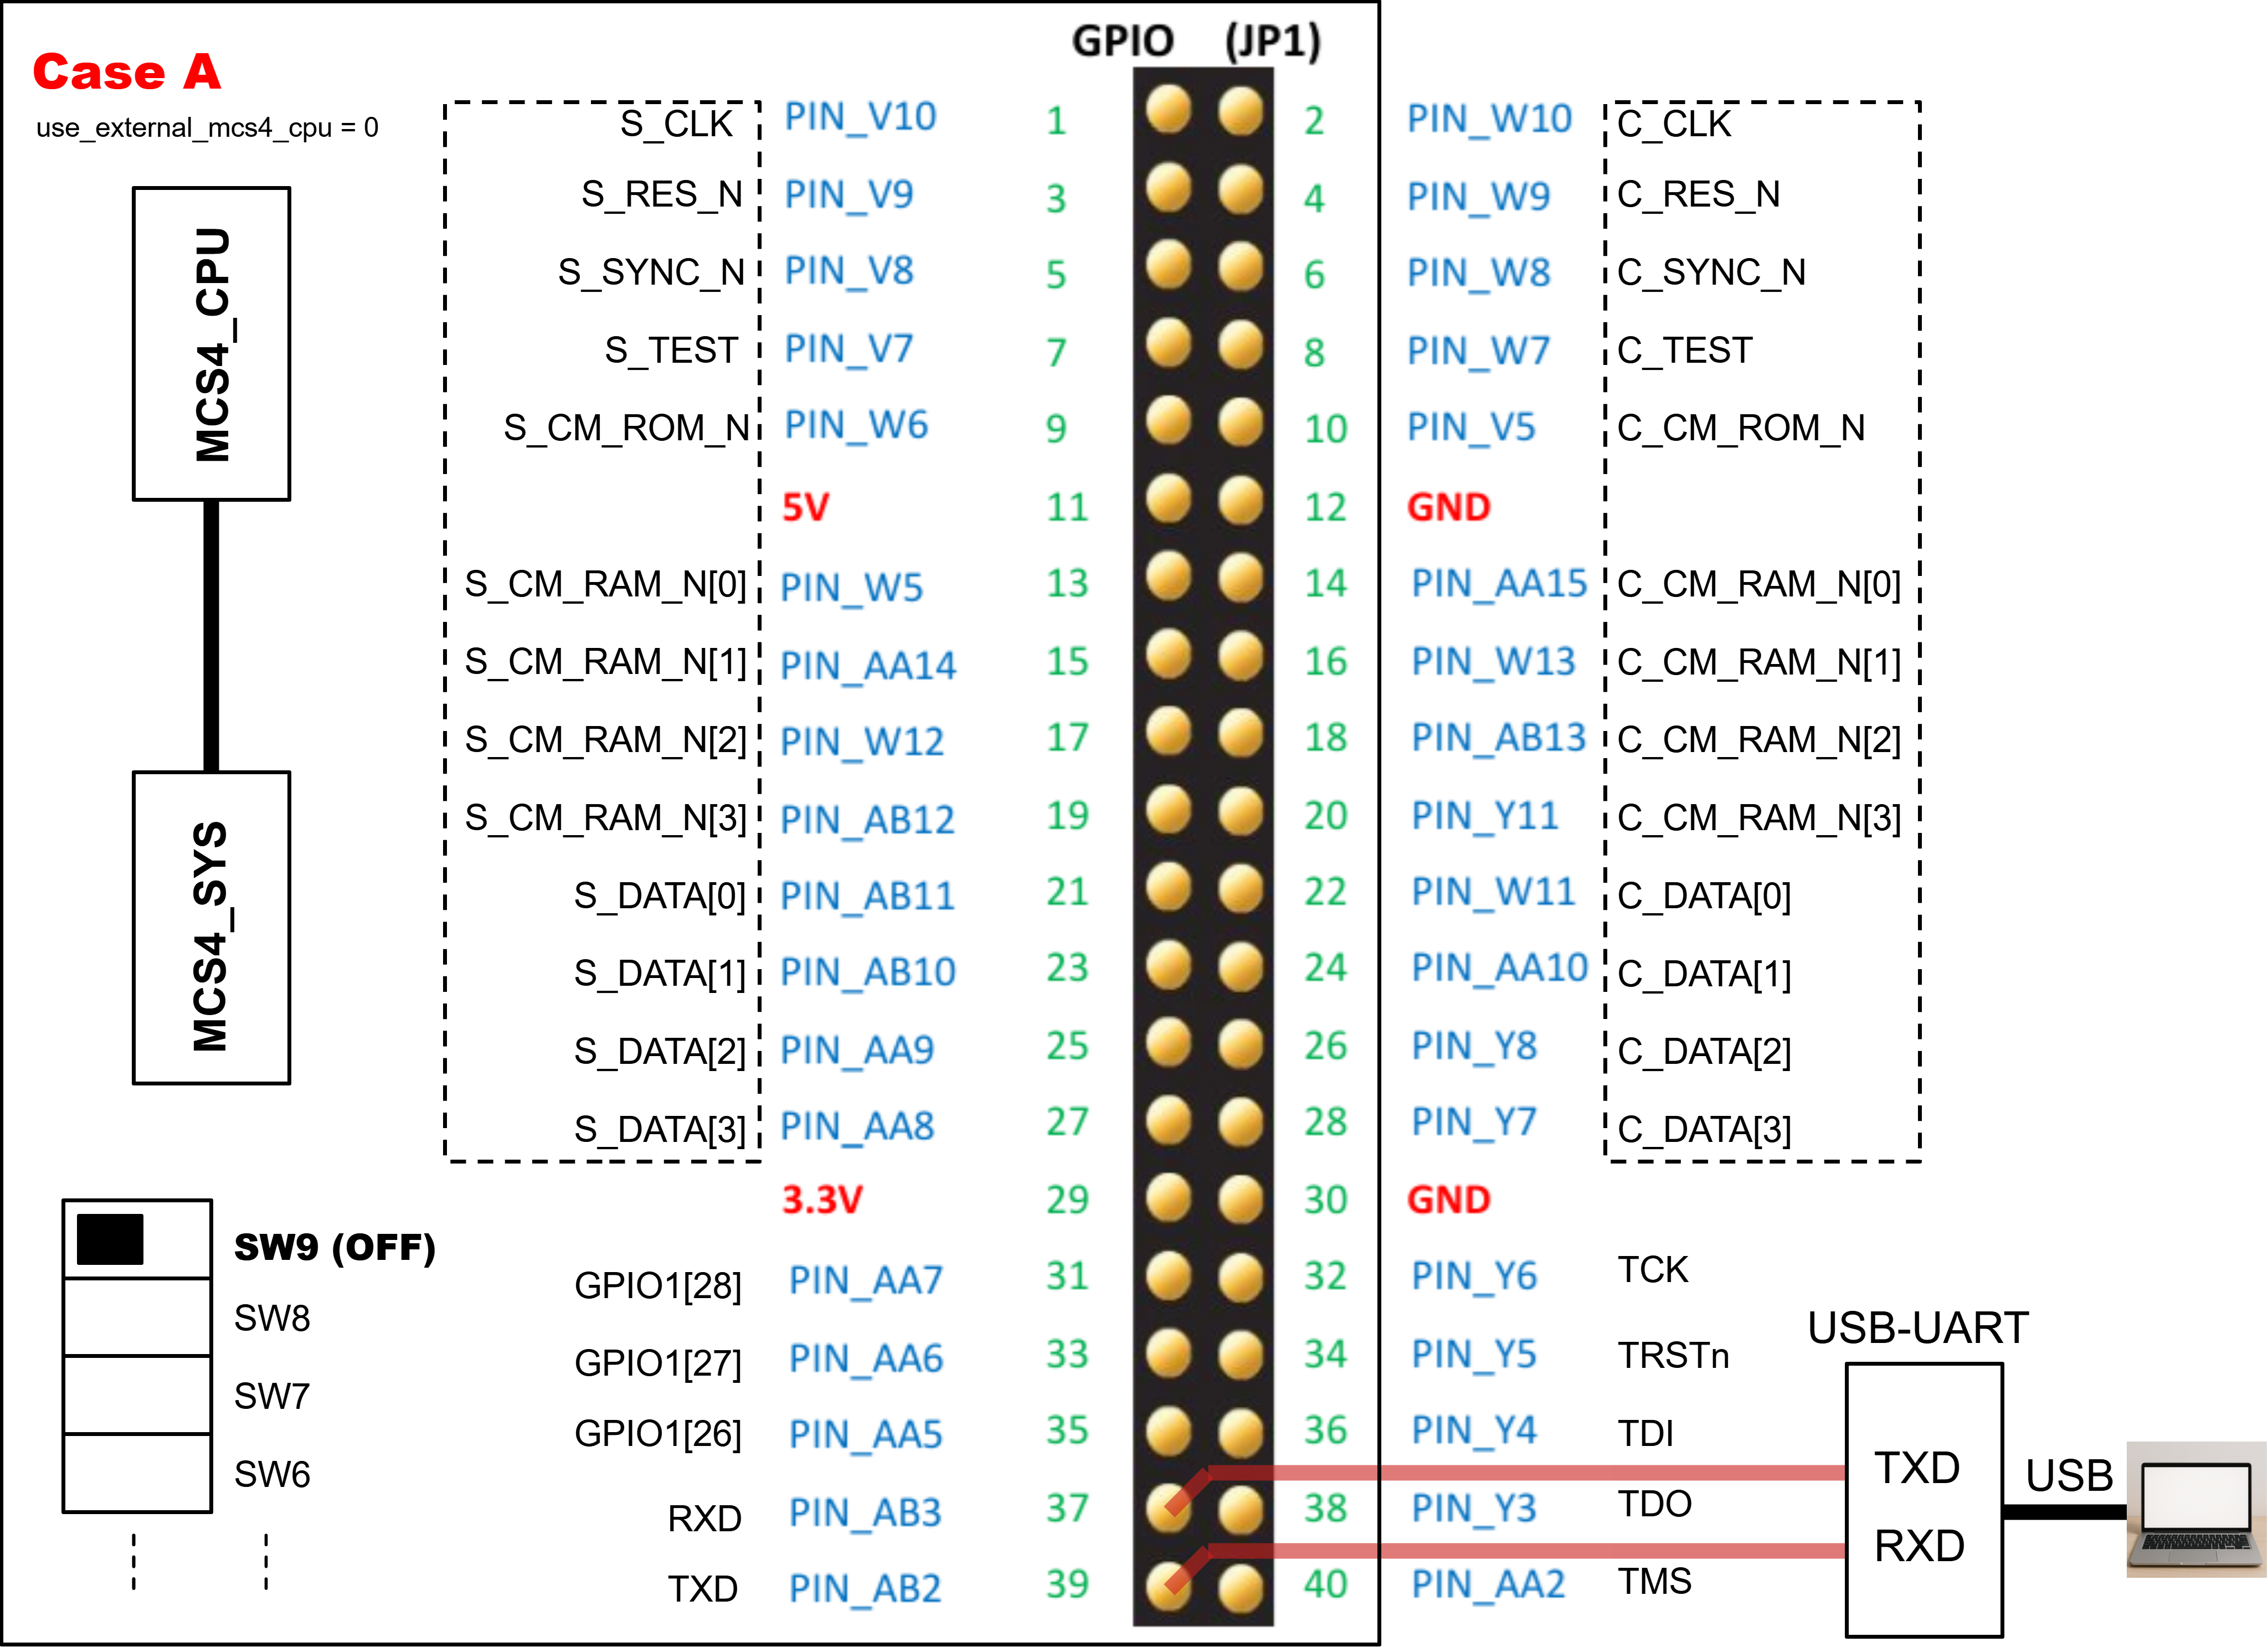
\includegraphics[width=0.75\textwidth]{./Figure/FPGACASEA.png}
  \caption{Case A:  MCS4\_CPU (4004 CPU) Connection}
  \label{fig:FPGACASEA}
\end{figure}
%----------------------------------
%----------------------------------
\begin{figure}[htbp]
  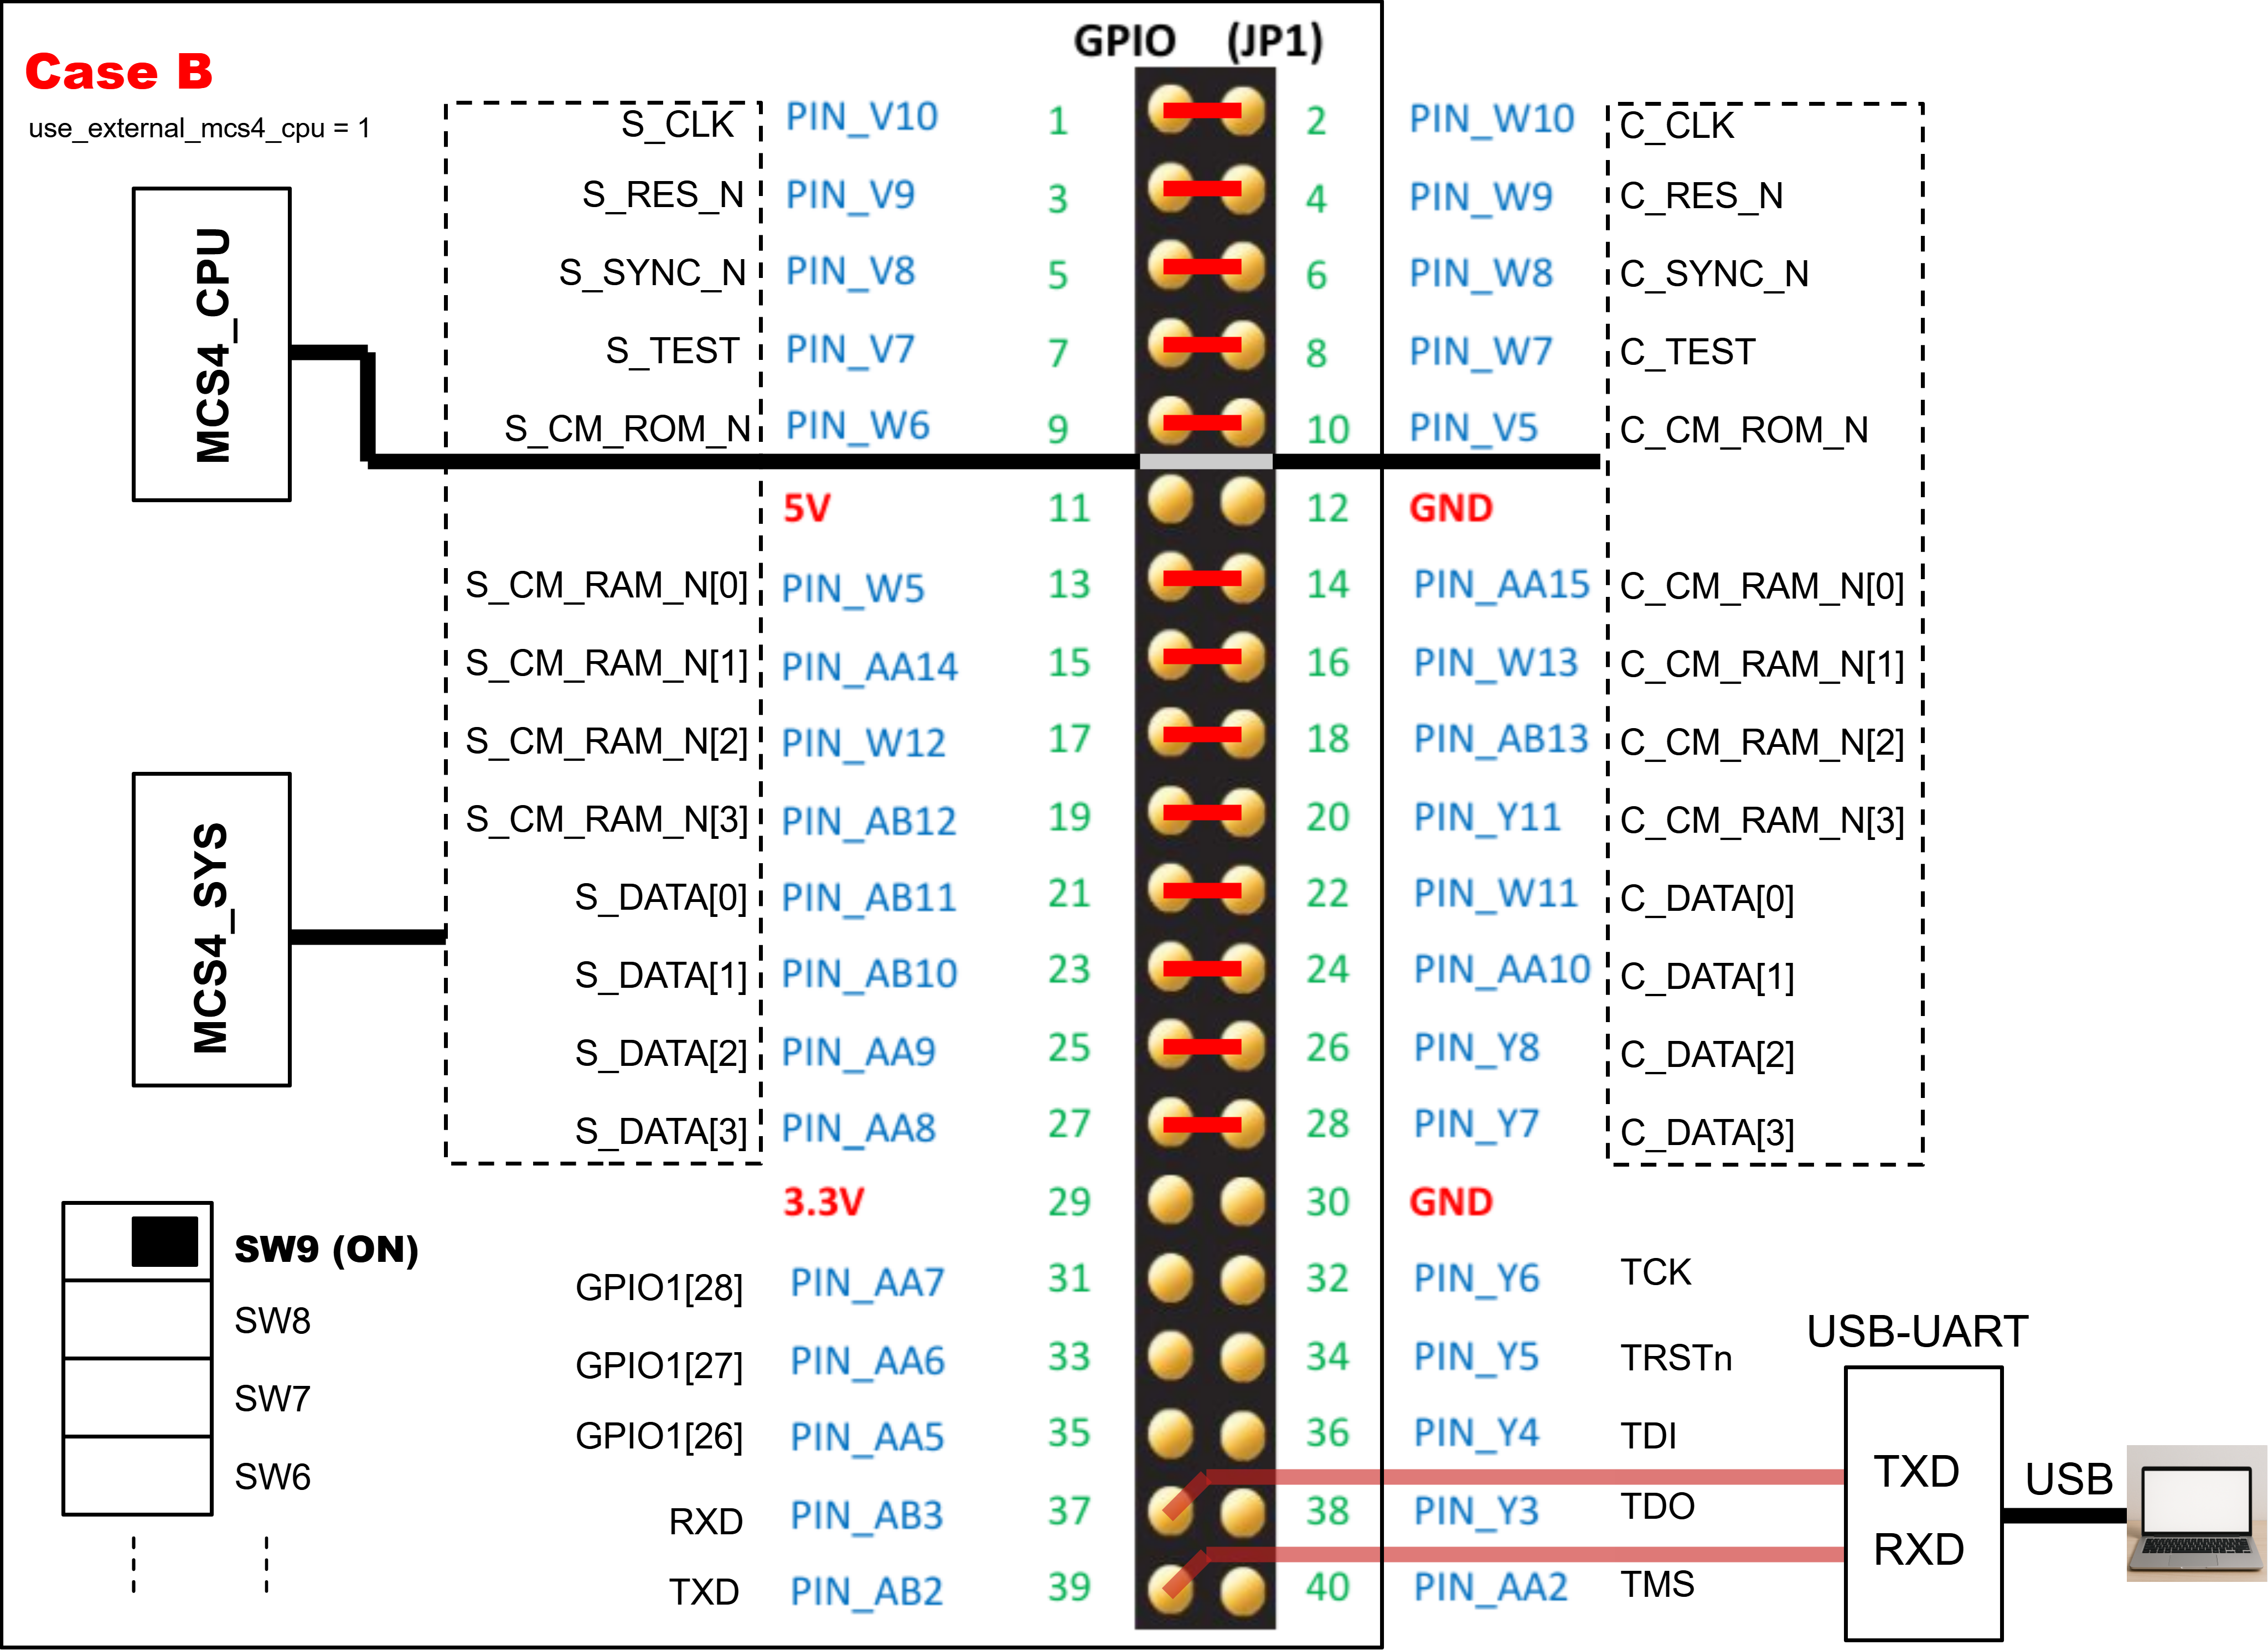
\includegraphics[width=0.75\textwidth]{./Figure/FPGACASEB.png}
  \caption{Case B:  MCS4\_CPU (4004 CPU) Connection}
  \label{fig:FPGACASEB}
\end{figure}
%----------------------------------
%----------------------------------
\begin{figure}[htbp]
  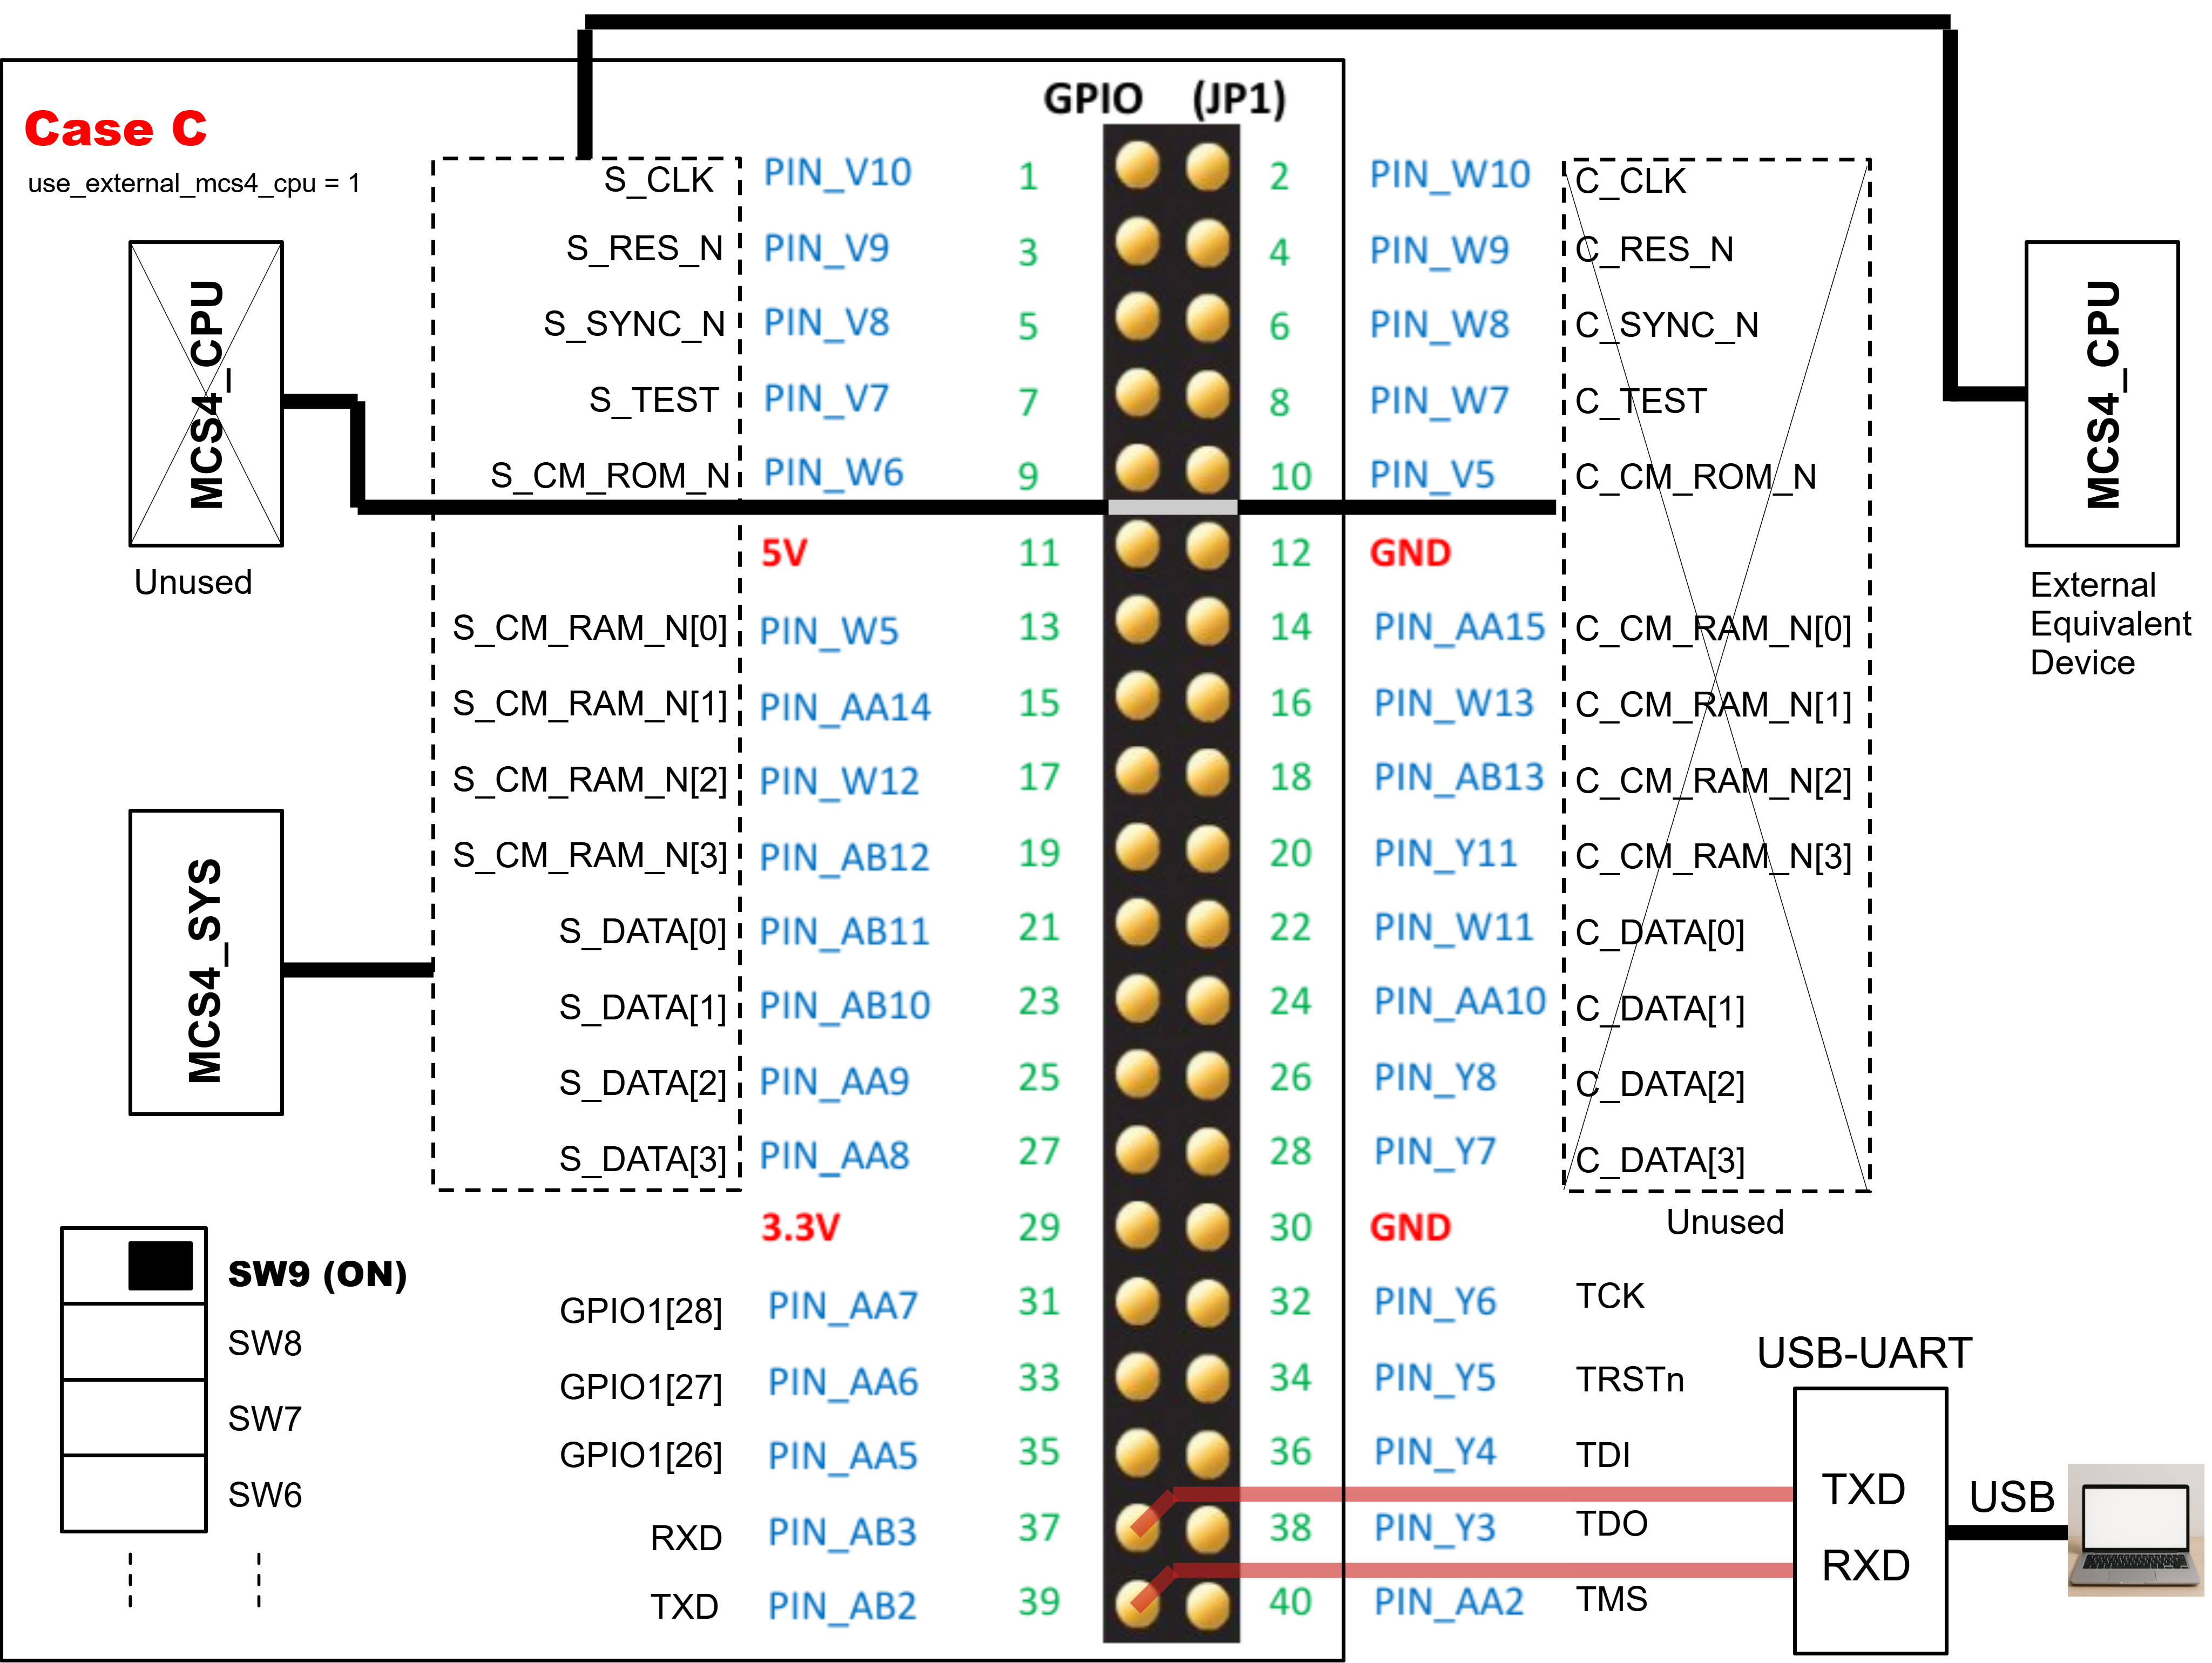
\includegraphics[width=0.75\textwidth]{./Figure/FPGACASEC.png}
  \caption{Case C:  MCS4\_CPU (4004 CPU) Connection}
  \label{fig:FPGACASEC}
\end{figure}
%----------------------------------

%--------------------------------------------------------------
\subsection{Connection for Debugging and Downloading RISC-V Programs}
To debug RISC-V programs from the integrated development environment Eclipse, download them to instruction memory, and execute them, connect the PC via the USB-JTAG interface board as shown in Figure~\ref{fig:FPGAJTAG}. A circuit example of the USB-JTAG interface board is depicted in Figure~\ref{fig:USBJTAG}. 

This interface board also provides USB-UART conversion functionality, enabling UART signals to be connected through it. For detailed methods of RISC-V debugging, please refer to the mmRISC-1 documentation~\cite{mmRISC-1}.

%----------------------------------
\begin{figure}[htbp]
  \includegraphics[width=0.75\textwidth]{./Figure/FPGAJTAG.png}
  \caption{Connection of RISC-V USB-JTAG Interface Board}
  \label{fig:FPGAJTAG}
\end{figure}
%----------------------------------
%----------------------------------
\begin{figure}[htbp]
  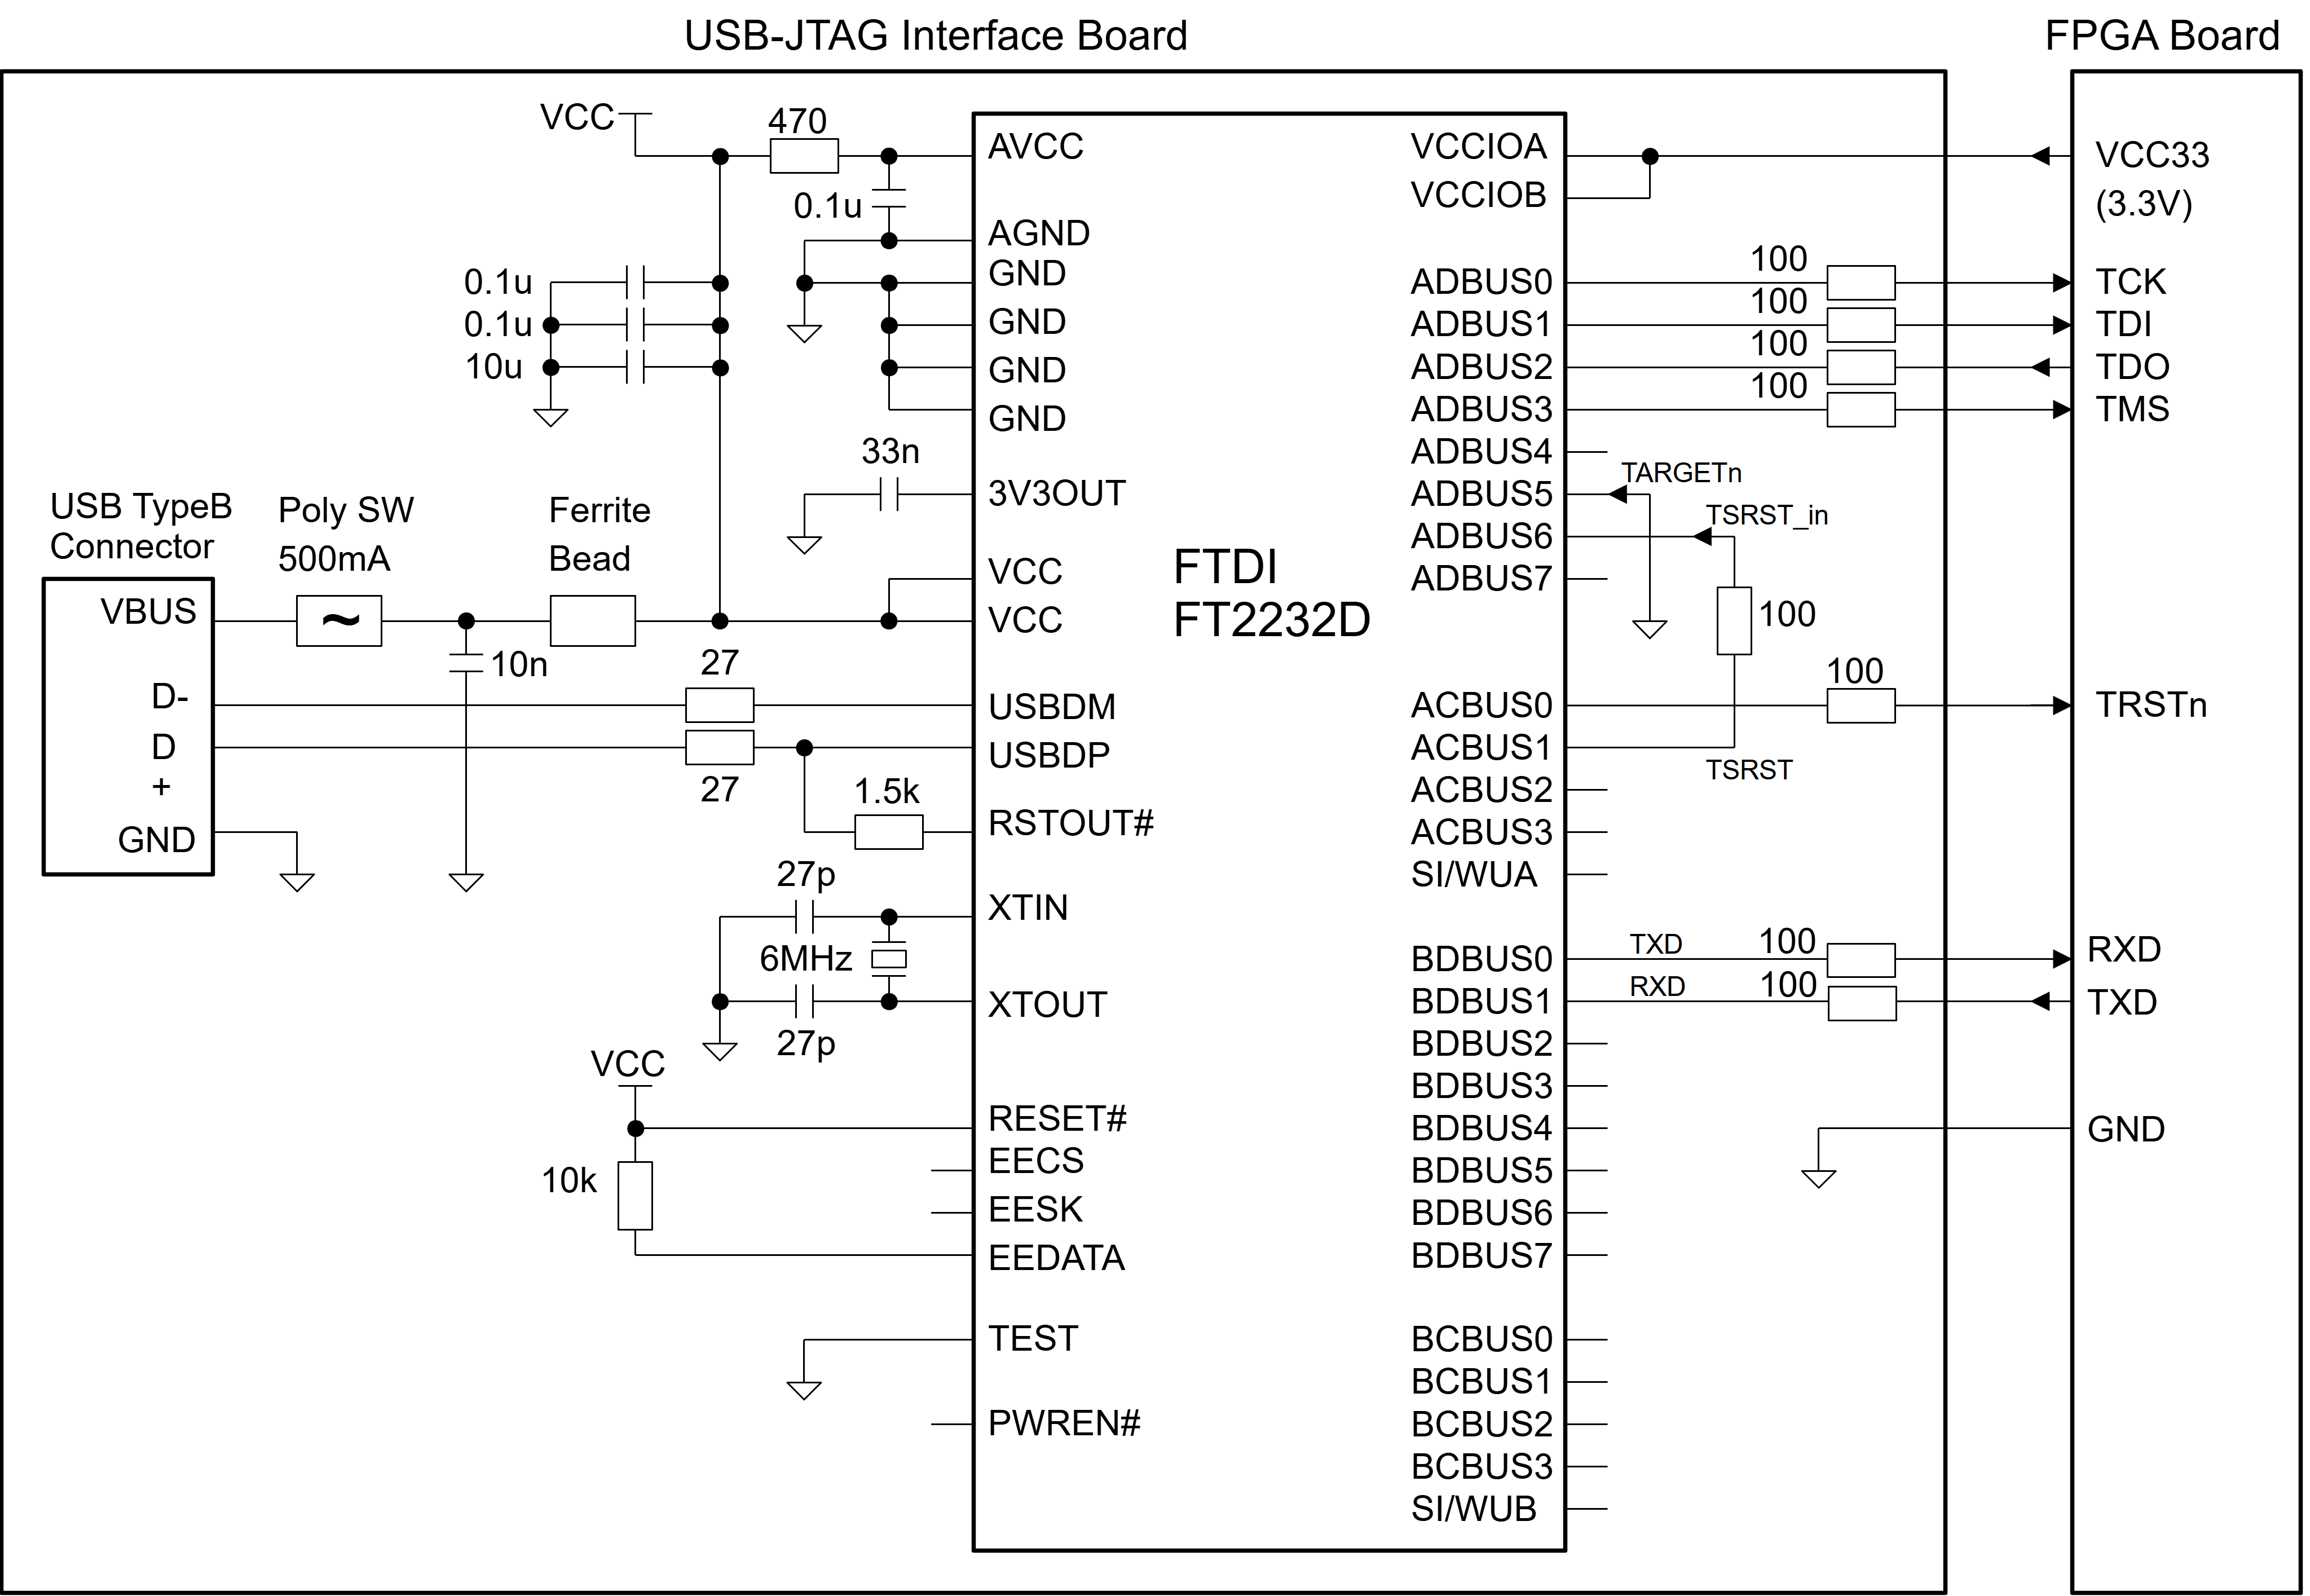
\includegraphics[width=0.75\textwidth]{./Figure/USBJTAG.png}
  \caption{An example of schematics of RISC-V USB-JTAG Interface Board}
  \label{fig:USBJTAG}
\end{figure}
%----------------------------------

%==============================================================
\section{Key Operation Method of the 141-PF Calculator}
Examples of key operation methods for the actual 141-PF calculator are shown in Figure~\ref{USAGE141PFCALC} and Figure~\ref{USAGE141PFMEM}.

Addition and subtraction behave slightly differently from modern calculators. Press the ``+'' or ``--'' key \emph{before} pressing the equal key. In other words, enter a value and then press ``+'' or ``--''. Please operate the keys as if saying aloud ``add the number'' or ``subtract the number''—and do just that.

Multiplication and division follow standard procedures found in contemporary calculators. \% Calculation, square root, and memory operations are handled similarly.

To input a negative number, press the ``S'' key before entering the numeric keys.

In the initial state, the number of digits after the decimal point is set to zero. Adjust the number of decimal places using the corresponding switches as needed. The rounding mode for the final digit can be selected via switch from the following options: Full significant digits display (FLOATING), round-off (ROUND), and truncation (TRUNCATE).

Additionally, three status indicator lamps are provided:
\begin{itemize}
  \item Overflow occurred (V)
  \item Negative result (N)
  \item Valid data stored in memory (M)
\end{itemize}

%----------------------------------
\begin{figure}[htbp]
  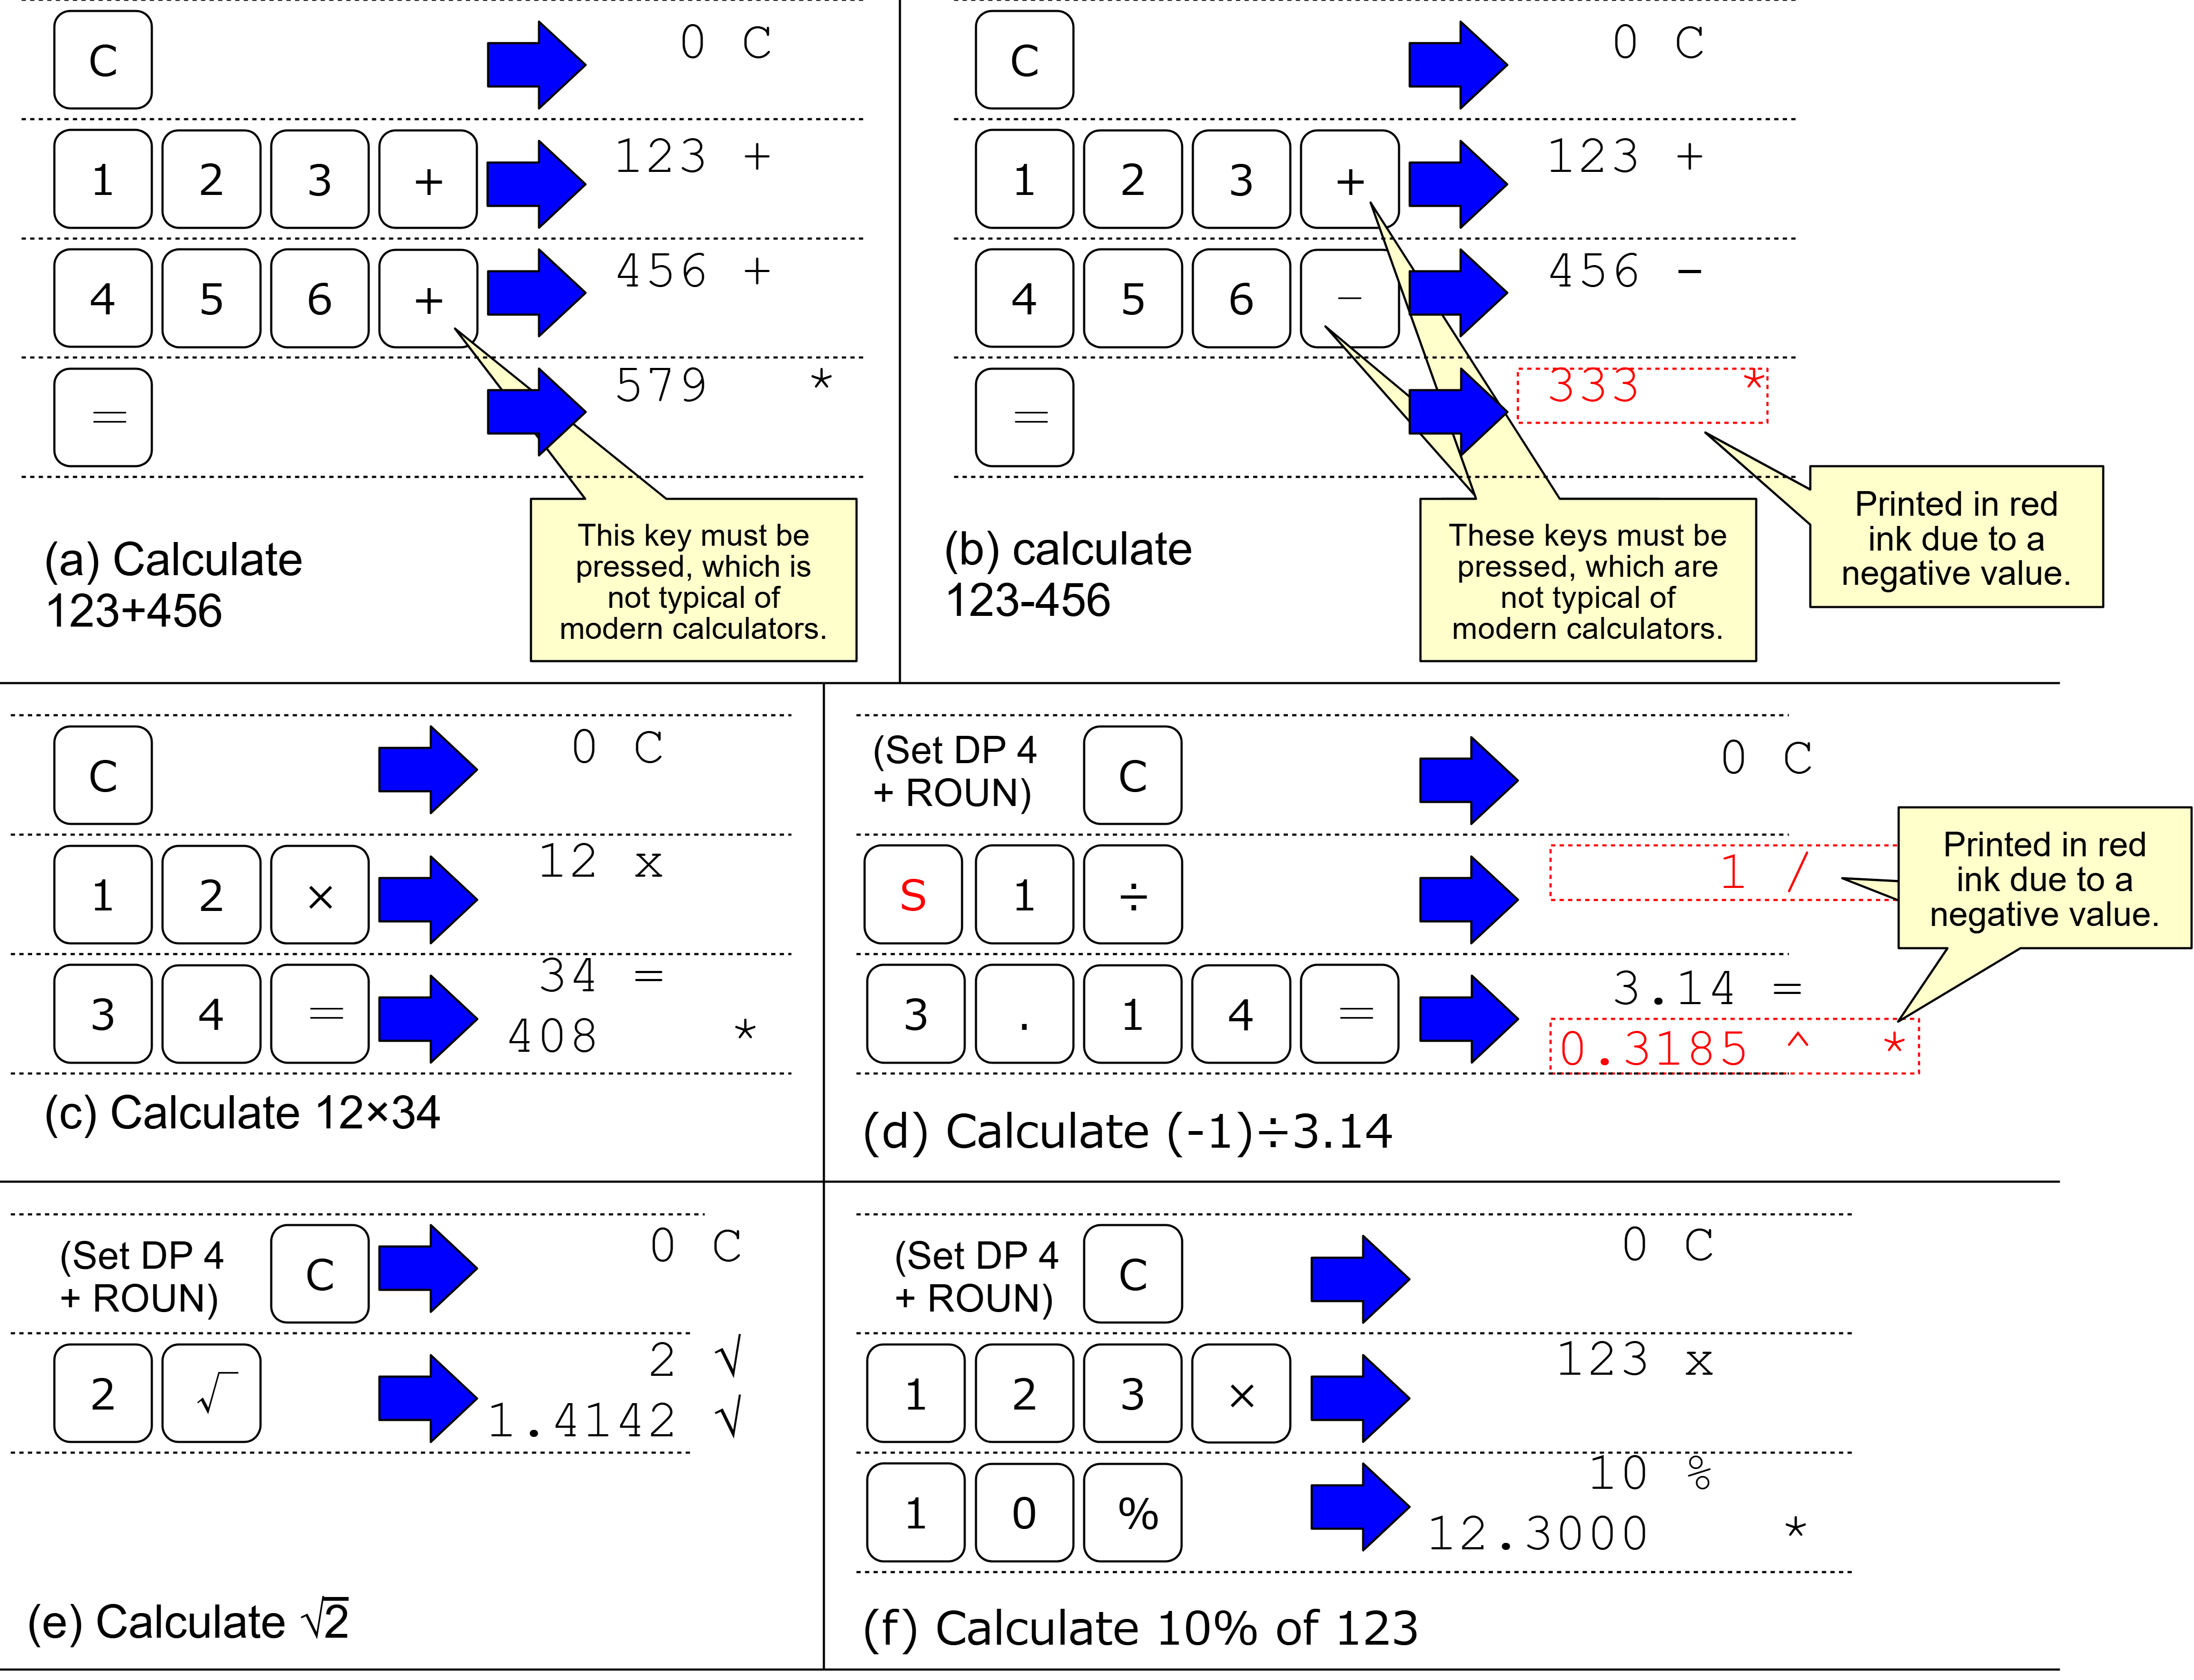
\includegraphics[width=1.0\textwidth]{./Figure/USAGE141PFCALC.png}
  \caption{How to use the 141-PF (Normal Calculation)}
  \label{fig:USAGE141PFCALC}
\end{figure}
%----------------------------------
%----------------------------------
\begin{figure}[htbp]
  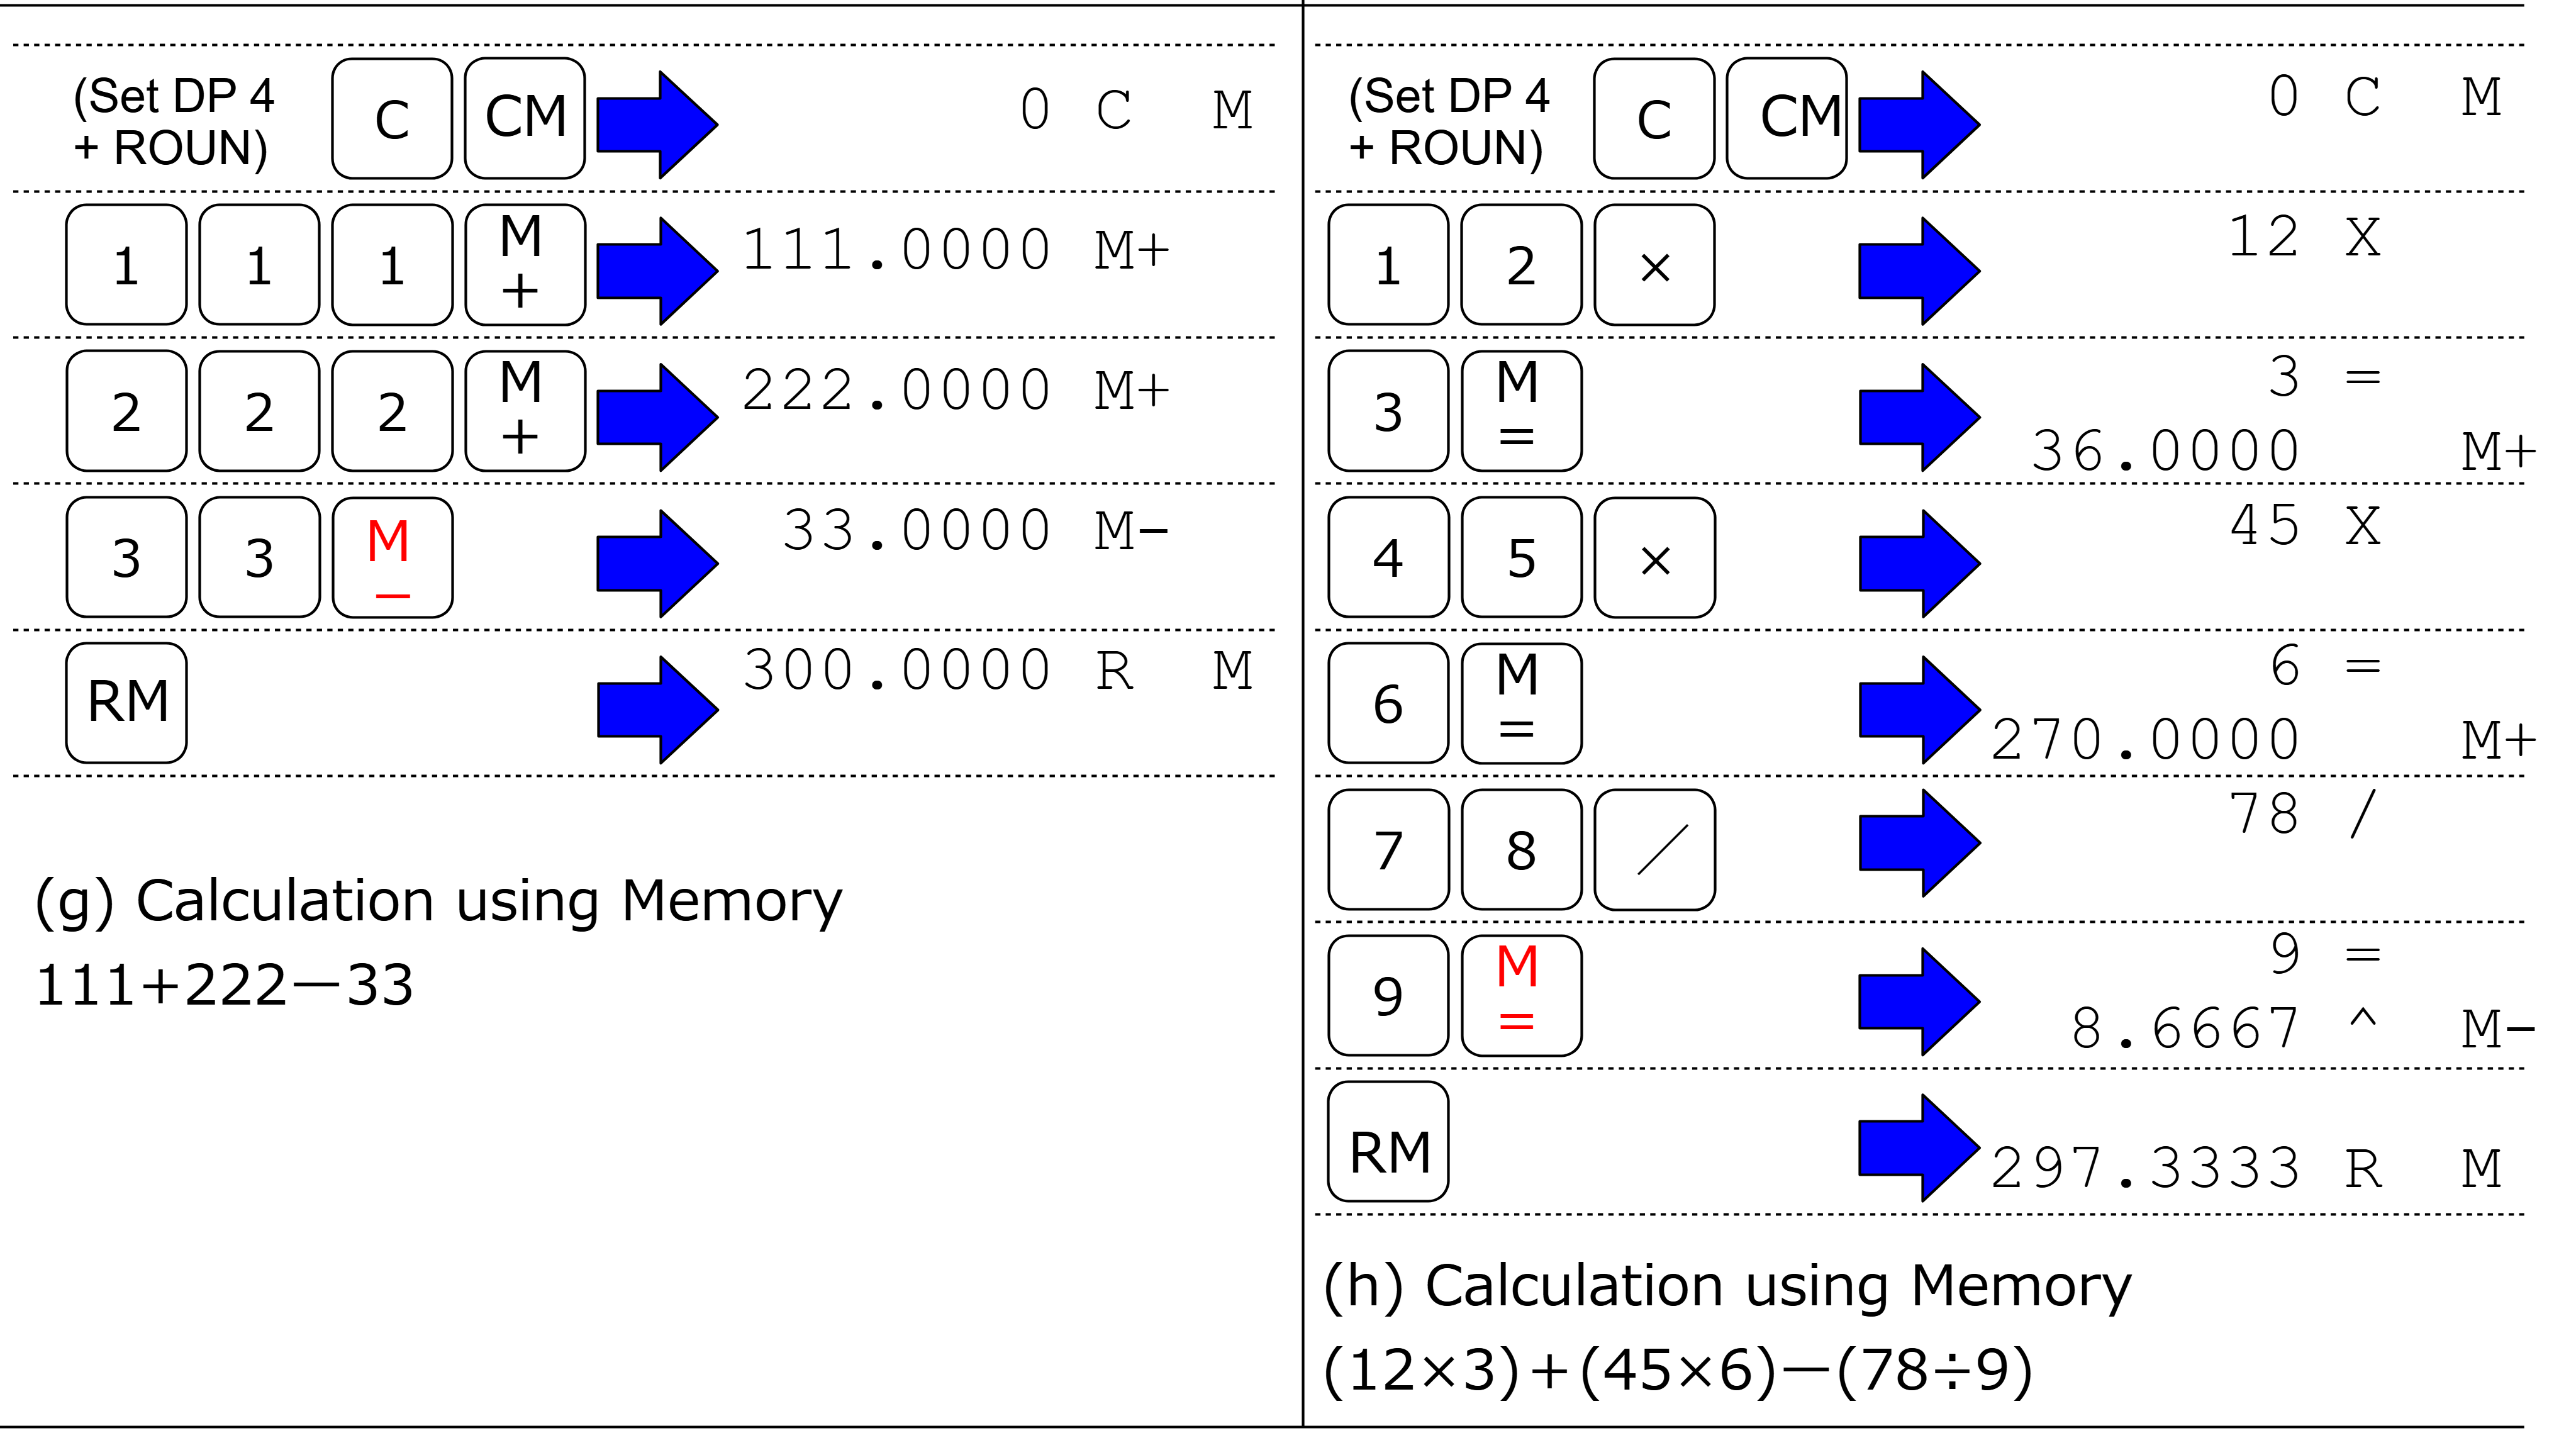
\includegraphics[width=1.0\textwidth]{./Figure/USAGE141PFMEM.png}
  \caption{How to use the 141-PF (Memory Calculation)}
  \label{fig:USAGE141PFMEM}
\end{figure}
%----------------------------------

%==============================================================
\section{The Charming Print Method of the 141-PF Calculator}

Unlike modern devices that display results on LCDs, VFDs, or LEDs, the Busicom 141-PF calculator printed its output on paper using a printer. The printer employed was Shinshu Seiki’s (now Seiko Epson) Model 102.

Inside the mechanism, a continuously rotating drum housed type characters embedded as reliefs. Above the drum were layers of paper, an ink ribbon, and a hammer. When the desired character on the drum rotated into alignment with the target print position, the hammer struck precisely, imprinting the character onto the paper.

On the calculator side, signals indicating the drum's rotational position were received, and for the characters most imminent on the drum, hammer signals were issued sequentially. As a result, digits in a print line did not appear left-to-right in order. Instead, the hammer struck various columns independently, and the full expression emerged as the print completed. This asynchronous yet elegant method delivers a truly unique and flavorful printing experience.

From an efficiency standpoint, this technique enabled the fastest possible printing with drum-style mechanisms. One cannot help but feel the determination and ingenuity of the engineers behind it.

The ink ribbon used a nostalgic two-color scheme of black and red, reminiscent of old mechanical typewriters. For each character, the ribbon's vertical position shifted to match the desired color. On the 141-PF calculator, negative values were printed in red.

%==============================================================
\section{Operation Method Using a Serial Terminal in This FPGA System}

This FPGA system was designed to replicate the operation of the Busicom 141-PF calculator. The following explains how to operate the system when using a serial terminal as the user interface.

The correspondence between the 141-PF calculator keys and characters entered from the terminal is shown in Table~\ref{tb:OPERATIONTERMINAL}. Instead of pressing a physical key, input the corresponding single character via the serial terminal. Note that the entered character does not appear on the terminal immediately—it is displayed in synchronization with the printer's timing, thereby emulating the flavorful behavior of the original drum-style printer.

%----------------------------------
\begin{table}[htbp]
    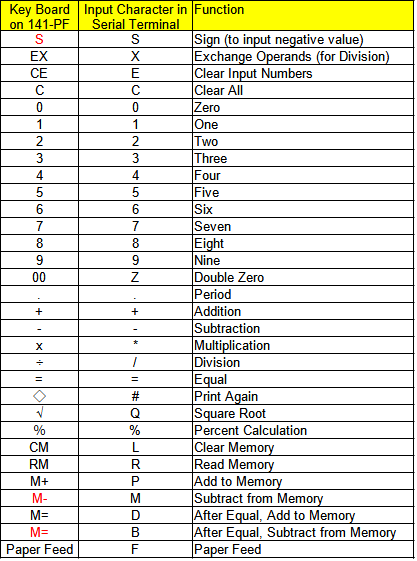
\includegraphics[width=0.5\columnwidth]{./Table/OperationTerminal.png}
    \caption{Operation of Key Input on Serial Terminal}
    \label{tb:OPERATIONTERMINAL}
\end{table}
%----------------------------------

To confirm the input from the terminal, the entered character is displayed on the seven-segment LED of the DE10-Lite board. While it is not possible to visually represent all letters or symbols accurately using seven segments, the format shown in Figure~\ref{fig:LED7SEG} is used for display.

%----------------------------------
\begin{figure}[htbp]
    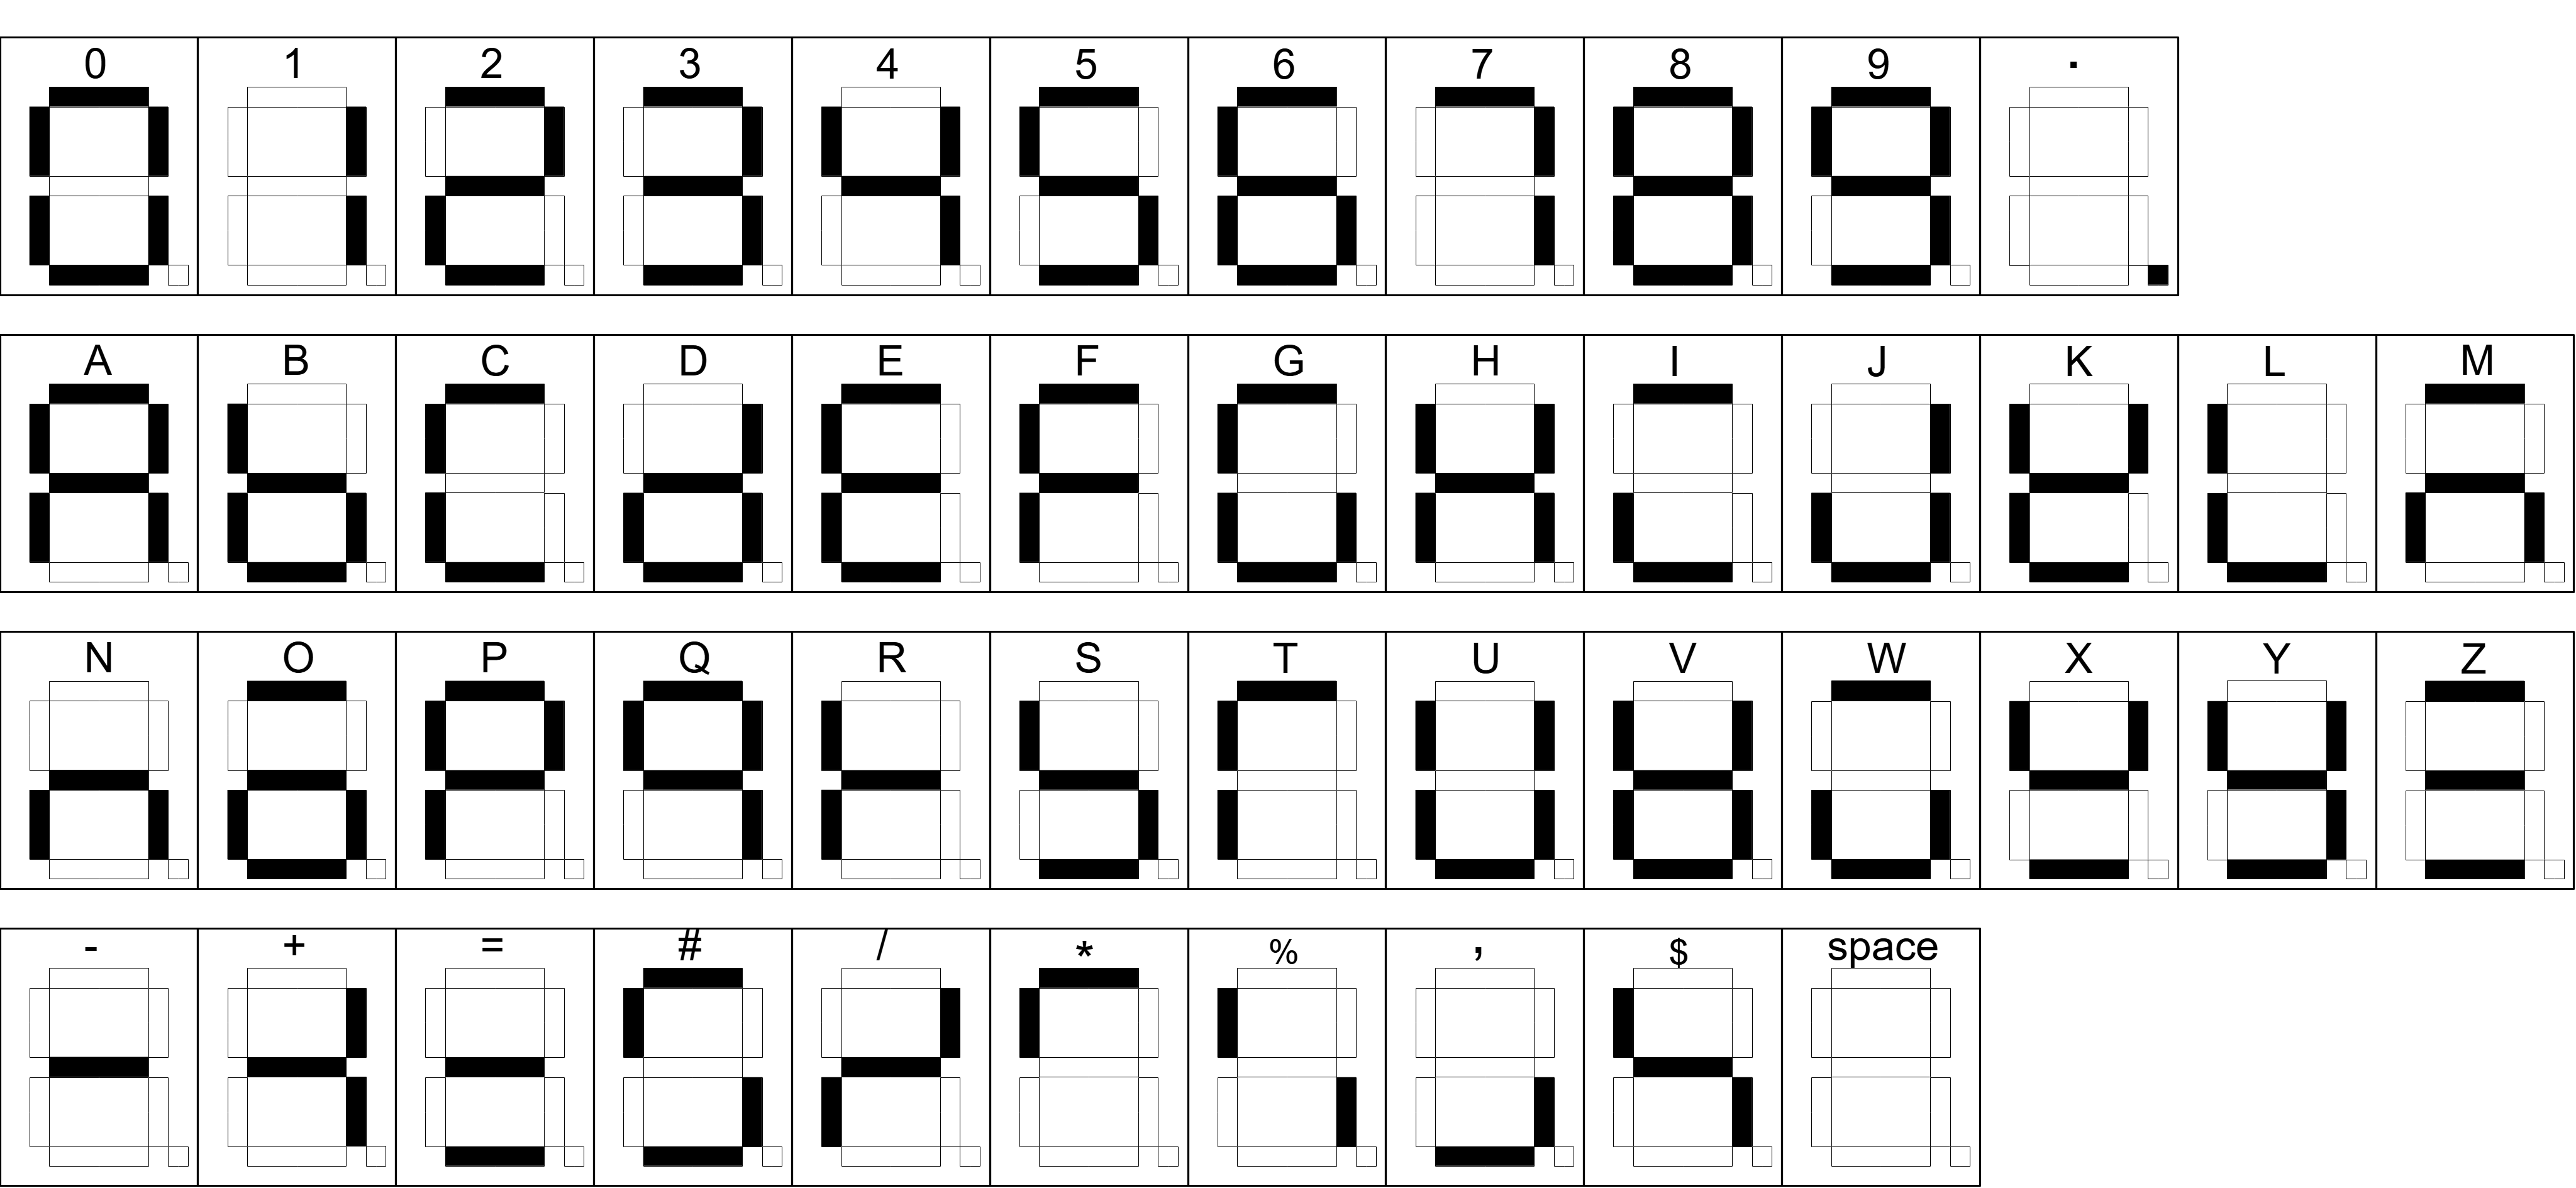
\includegraphics[width=1.0\columnwidth]{./Figure/LED7SEG.png}
    \caption{Character Display on 7 segment LED}
    \label{fig:LED7SEG}
    \textit{The seven-segment LED display format was inspired by the console representation used in Hitachi’s 8-bit microcomputer 6800 training kit H68/TR, with some extensions made to suit this system.}\\
    \scriptsize{\url{https://www.hitachihyoron.com/jp/pdf/1977/05/1977_05_12.pdf}}
\end{figure}
%----------------------------------

To operate the decimal point and rounding switches, input the ``ESC'' character on the serial terminal. This triggers the following configuration prompts, where you can set each option. Once both configurations are completed, the system will return to the key input standby state.

\begin{scriptsize}
\begin{boxedverbatim}
----------------------------
Set Slide Switches on 141-PF
----------------------------
Decimal Point : 0~6/8 (now 1)=? 
Decimal Point SW Not Changed (now 1)
Rounding : FLOT=0/ROUN=1/TRNC=8 (now 0)=? 1
Rounding SW Changed (now 1)
----------------------------
\end{boxedverbatim}
\end{scriptsize}
\\

Since the serial terminal cannot display red characters, lines that include red-printed values are marked with a [RED] tag at the end of the line. Additionally, the status indicators—overflow (V), negative result (N), and valid memory data (M)—are also displayed at the end of each line.\\

On the DE10-Lite board, LEDR0 through LEDR9 display the upper 10 bits (PC[11:2]) of the program counter (PC) of the MCS4\_CPU (4004 CPU). This allows you to observe how the instruction address of the currently running program changes over time.

%==============================================================
\section{Operation Method Using the Touch LCD Shield in This FPGA System}

When the touch LCD shield is mounted on the designed FPGA, the graphical user interface allows intuitive operation as shown in Figure~\ref{fig:OPERATIONTOUCHLCD}. This interface also faithfully reproduces the charming behavior of the original drum-style printer from the Busicom 141-PF calculator.

Touching the **left half of the print area** brings up a configuration window for controlling the **decimal point switch** and the **rounding switch**. Touching the **right half of the print area** performs a **paper feed** operation.

When each key is tapped on the touchscreen, the input character corresponding to the key is also shown on the **seven-segment LED** of the DE10-Lite board—just as in serial terminal operation. While seven-segment displays have limitations in expressing certain symbols and letters, this visual feedback supports confirmation of input.\\

Note that all touchscreen operations are designed to match the tactile feedback and timing of the original machine, preserving the authentic retrocomputing experience such as printing sequence of drum printer.\\

Just same as the serial terminal mode, on the DE10-Lite board, LEDR0 through LEDR9 display the upper 10 bits (PC[11:2]) of the program counter (PC) of the MCS4\_CPU (4004 CPU). This allows you to observe how the instruction address of the currently running program changes over time.

%----------------------------------
\begin{figure}[htbp]
    \includegraphics[width=1.0\columnwidth]{./Figure/OperationTouchLCD.png}
    \caption{Operation on Touch LCD Panel}
    \label{fig:OPERATIONTOUCHLCD}
\end{figure}
%----------------------------------

%==============================================================





